\chapter{Neutrino Oscillation Physics}
\label{chap:NeutrinoOscillationPhysics}

When first proposed, neutrinos were expected to be approximately massless fermions that only interact through weak and gravitational forces. This meant they were very difficult to detect as they can pass through significant amounts of matter without interacting. Despite this, experimental neutrino physics has developed many different detection techniques and observed neutrinos from both natural and artificial sources. In direct tension with Standard Model physics, neutrinos have been determined to oscillate between different lepton flavours, requiring them to have mass. 

The observation techniques which led to the discovery of the neutrino are documented in \autoref{sec:NeutrinoOscillationPhysics_Discovery}. The theory underpinning neutrino oscillation is described in \autoref{sec:NeutrinoOscillationPhysics_EvidenceForNeutrinoOscillation} and includes the approximations which can be made to simplify the understanding of neutrino oscillation in the two-flavour approximation. Past, current, and future neutrino experiments are detailed in \autoref{sec:NeutrinoOscillationPhysics_OscillationMeasurements}, including the reactor, atmospheric, and long-baseline accelerator neutrino sources that have been used to successfully constrain oscillation parameters. Finally, the current state of oscillation parameter measurements are summarised in \autoref{sec:Theory_Summary}.

\section{Discovery of Neutrinos}
\label{sec:NeutrinoOscillationPhysics_Discovery}

At the start of the \quickmath{20^{th}} century, the electrons emitted from the \quickmath{\beta}-decay of the nucleus were found to have a continuous energy spectrum \cite{Chadwick:262756, Ellis1927-qf}. This observation seemingly broke the energy conservation invoked within that period's nuclear models. In 1930, Pauli provided a solution to this problem in the form of a new particle, the neutrino (originally termed ``neutron''). It was theorized to be an electrically neutral spin-\quickmath{1/2} fermion with a mass smaller than that of the electron \cite{Pauli:1930pc}. This neutrino was emitted with the electron in \quickmath{\beta}-decay to alleviate the apparent breaking of energy conservation. As a predecessor of today's weak interaction model, Fermi's theory of \quickmath{\beta}-decay developed the understanding by coupling the four constituent particles: electron, proton, neutron, and neutrino, into a quantitative model \cite{Fermi:1934hr}.

Whilst Pauli was not convinced of the ability to detect neutrinos, the first observations of the particle were made in the mid-1950s when neutrinos from a reactor were observed via the inverse \quickmath{\beta}-decay (IBD) process, \quickmath{\bar{\nu}_{e} + p \rightarrow n + e^{+}} \cite{reines_cowan_1,reines_cowan_2}.
%The detector consisted of cadium-doped water targets surronded by liquid scintillator, which was monitored by a suite of photo-multiplier tubes.
The detector consisted of two parts: a neutrino interaction medium and a liquid scintillator. The interaction medium was built from two water tanks, loaded with cadmium chloride to allow for increased efficiency in the detection of neutron capture. The positron emitted from IBD annihilates, \quickmath{e^{+} + e^{-} \rightarrow 2\gamma}, generating a prompt signal and the neutron is captured on the cadmium via \quickmath{n + ^{108}Cd \rightarrow ^{109*}Cd \rightarrow ^{109}Cd + \gamma}, producing a delayed signal. An increase in the coincidence rate was observed when the reactor was operating which was interpreted as interactions from neutrinos generated in the reactor.

After the discovery of the \quickmath{\nu_{e}}, the question of how many flavours of neutrino exist was asked. In 1962, a measurement of the \quickmath{\nu_{\mu}} was conducted at the Brookhaven National Laboratory \cite{Lederman}. A proton beam was directed at a beryllium target, generating pions which then decayed via \quickmath{\pi^{\pm} \rightarrow \mu^{\pm} + (\nu_{\mu}, \bar{\nu}_\mu}), and the subsequent interactions of the \quickmath{\nu_{\mu}} were observed. As the subsequent interaction of the neutrino generated muons rather than electrons, it was determined that the \quickmath{\nu_{\mu}} was fundamentally different from \quickmath{\nu_{e}}. The final observation to be made was that of the \quickmath{\nu_{\tau}} from the DONUT experiment \cite{tau_nu_disc}. Three neutrinos seem the obvious solution as it mirrors the known number of charged leptons (as they form weak isospin doublets) but there could be evidence of more. Several neutrino experiments have found anomalous results \cite{PhysRevD.64.112007, PhysRevLett.110.161801} which could be attributed to ``sterile'' neutrinos. These hypothesised particles are not affected by gauge interactions in the Standard Model so their presence can only be inferred through the observation of non-standard oscillation modes. However, cosmological observations indicate the number of neutrino species \quickmath{N_{eff} = 2.99 \pm 0.17} \cite{Planck2018}, as measured from the cosmic microwave background power spectrum. LEP also measured the number of active neutrino flavours to be \quickmath{N_{\nu} = 2.9840 \pm 0.0082} \cite{lep} from measurements of the Z-decay width, but this does not strongly constrain the number of sterile neutrinos.

\section{Theory of Neutrino Oscillation}
\label{sec:NeutrinoOscillationPhysics_EvidenceForNeutrinoOscillation}

%As direct evidence of beyond Standard Model physics,
%(as seen in \autoref{sec:NeutrinoOscillationPhysics_3FlavourOsc}).
%This observation is direct evidence of beyond Standard Model physics.
A neutrino generated with lepton flavour \quickmath{\alpha} can change into a different lepton flavour \quickmath{\beta} after propagating some distance. This phenomenon is called neutrino oscillation and requires that neutrinos must have a non-zero mass. This behaviour has been characterised by the Pontecorvo-Maki-Nakagawa-Sakata (PMNS) \cite{p1,p2,km} mixing matrix which describes how the flavour and mass of neutrinos are associated. This is analogous to the Cabbibo-Kobayashi-Maskawa (CKM) \cite{cabbibo} matrix measured in quark physics.

\subsection{Three Flavour Oscillations}
\label{sec:NeutrinoOscillationPhysics_3FlavourOsc}

The PMNS parameterisation defines three flavour eigenstates, \quickmath{\nu_{e}}, \quickmath{\nu_{\mu}} and \quickmath{\nu_{\tau}} (indexed \quickmath{\nu_{\alpha}}), which are eigenstates of the weak interaction and three mass eigenstates, \quickmath{\nu_{1}}, \quickmath{\nu_{2}} and \quickmath{\nu_{3}} (indexed \quickmath{\nu_{i}}). Each mass eigenstate is the superposition of all three flavour states,

\begin{equation}
  \label{eq:NeutrinoOscillationPhysics_Superposition}
  \left|\nu_{i}\right> = \sum_{\alpha}\mathrm{U}_{\alpha i}\left|\nu_{\alpha}\right>.
\end{equation}

Where \quickmath{\mathrm{U}} is the \quickmath{3 \times 3} PMNS matrix which is unitary and connects the mass and flavour eigenstates.

%
\iffalse
\begin{equation}
  \label{eq:NeutrinoOscillationPhysics_PMNSReduced}
  \mathrm{U} = \begin{pmatrix} \mathrm{U}_{e1} & \mathrm{U}_{e2} & \mathrm{U}_{e3} \\ \mathrm{U}_{\mu 1} & \mathrm{U}_{\mu 2} & \mathrm{U}_{\mu 3} \\ \mathrm{U}_{\tau 1} & \mathrm{U}_{\tau 2} & \mathrm{U}_{\tau 3} \end{pmatrix}.
\end{equation}
\fi
%

The weak interaction, when interacting via a \quickmath{W^{\pm}} boson, couples to flavour eigenstates so neutrinos interact with leptons of the same flavour. The propagation of a neutrino flavour eigenstate, in a vacuum, can be re-written as a plane-wave solution to the time-dependent Schr{\"o}dinger equation,

\begin{equation}
  \label{eq:NeutrinoOscillationPhysics_TimeDepSuperposition}
  \left|\nu_{\alpha}(t)\right> = \sum_{i}\mathrm{U}^{*}_{\alpha i}\left|\nu_{i}\right>e^{-i \phi_{i}}.
\end{equation}

The \quickmath{\phi_{i}} term can be expressed in terms of the energy, \quickmath{E_{i}}, and magnitude of the three momenta, \quickmath{p_{i}}, of the neutrino, \quickmath{\phi_{i} = E_{i}t - p_{i}x} (\quickmath{t} and \quickmath{x} being time and position coordinates). The probability of observing a neutrino of flavour eigenstate \quickmath{\beta} from one which originated as flavour \quickmath{\alpha} can be calculated as,

\begin{equation}
  \label{eq:NeutrinoOscillationPhysics_ProbabilityComplexForm}
  P(\nu_{\alpha} \rightarrow \nu_{\beta}) = \left| \left< \nu_{\beta} | \nu_{\alpha}(t) \right> \right|^{2} = \sum_{i,j} \mathrm{U}^{*}_{\alpha i}\mathrm{U}_{\beta i}\mathrm{U}_{\alpha j}\mathrm{U}^{*}_{\beta j} e^{-i(\phi_{j}-\phi_{i})}.
\end{equation}

The term within the exponential can be represented as,

\begin{equation}
  \label{eq:NeutrinoOscillationPhysics_PhaseDifference}
  \phi_{j}-\phi_{i} = E_{j}t - E_{i}t - p_{j}x + p_{i}x .
\end{equation}

For a relativistic particle, \quickmath{E_{i} \gg m_{i}}, a Taylor series expansion means,

\begin{equation}
  p_{i} = \sqrt{E^{2}_{i} - m^{2}_{i}} \approx E_{i} - \frac{m^{2}_{i}}{2E_{i}}.
\end{equation}

Making the approximations that neutrinos are relativistic, the mass eigenstates were created with the same energy and that \quickmath{x = L}, where \quickmath{L} is the distance travelled by the neutrino, \autoref{eq:NeutrinoOscillationPhysics_PhaseDifference} then becomes

\begin{equation}
  \phi_{j}-\phi_{i} = \frac{\Delta m^{2}_{ij} L}{2E},
\end{equation}

where \quickmath{\Delta m^{2}_{ij} = m^{2}_{i} - m^{2}_{j}}. This, combined with further use of unitarity relations results in \autoref{eq:NeutrinoOscillationPhysics_ProbabilityComplexForm} becoming

\begin{equation}
  \label{eq:NeutrinoOscillationPhysics_ProbabilityComplexForm2}
  \begin{split}
    P(\nu_{\alpha} \rightarrow \nu_{\beta}) &= \delta_{\alpha \beta} - 4 \sum_{i>j} \mathbb{R} \left( \mathrm{U}^{*}_{\alpha i}\mathrm{U}_{\beta i}\mathrm{U}_{\alpha j}\mathrm{U}^{*}_{\beta j} \right) \sin^{2} \left( \frac{\Delta m^{2}_{ij} L}{4E} \right) \\
    & + \left( - \right) 2 \sum_{i>j} \mathbb{I} \left( \mathrm{U}^{*}_{\alpha i}\mathrm{U}_{\beta i}\mathrm{U}_{\alpha j}\mathrm{U}^{*}_{\beta j} \right) \sin \left( \frac{\Delta m^{2}_{ij} L}{2E} \right). \\
    \end{split}
\end{equation}

Where \quickmath{\delta_{\alpha \beta}} is the Kronecker delta function and the negative sign on the last term is included for the oscillation probability of antineutrinos. As an important point to note, the observation of oscillation probability requires a non-zero value of \quickmath{\Delta m^{2}_{ij}}, which in turn requires that neutrinos have differing masses.

Typically, the PMNS matrix is parameterised into three mixing angles, a charge parity (CP) violating phase \quickmath{\delta_{CP}}, and two Majorana phases \quickmath{\alpha_{1,2}},

\begin{equation}
  \label{eq:NeutrinoOscillationPhysics_PMNS}
  \begin{split}
  \mathrm{U} =
  \underbrace{\begin{pmatrix} 1 & 0 & 0 \\ 0 & c_{23} & s_{23} \\ 0 & -s_{23} & c_{23} \end{pmatrix}}_{\text{Atmospheric, Accelerator}} &
  \underbrace{\begin{pmatrix} c_{13} & 0 & s_{13}e^{-i \delta_{CP}} \\ 0 & 1 & 0 \\ -s_{13}e^{-i \delta_{CP}} & 0 & c_{13} \end{pmatrix}}_{\text{Reactor, Accelerator}} \\
  & \times \underbrace{\begin{pmatrix} c_{12} & s_{12} & 0 \\ -s_{12} & c_{12} & 0 \\ 0 & 0 & 1 \end{pmatrix}}_{\text{Reactor, Solar}}
  \underbrace{\begin{pmatrix} e^{i\alpha_{1}/2} & 0 & 0 \\ 0 & e^{i\alpha_{2}/2} & 0 \\ 0 & 0 & 1 \end{pmatrix}}_{\text{Majorana}}.
  \end{split}
\end{equation}

Where \quickmath{s_{ij} = \sin(\theta_{ij})} and \quickmath{c_{ij} = \cos(\theta_{ij})}. The oscillation parameters are often grouped: \quickmath{(1,2)} as ``solar'', \quickmath{(2,3)} as ``atmospheric'' and \quickmath{(1,3)} as ``reactor''. Many neutrino experiments aim to measure the PMNS parameters from a wide array of origins, as is the purpose of this thesis.

The Majorana phase, \quickmath{\alpha_{1,2}}, included within the fourth matrix in \autoref{eq:NeutrinoOscillationPhysics_PMNS} is only included for completeness. For an oscillation analysis experiment, any terms containing this phase disappear due to taking the expectation value of the PMNS matrix. Measurements of these phases can be performed by experiments searching for neutrino-less double \quickmath{\beta}-decay \cite{Maio_2015}.

A two-flavour approximation can be obtained when one assumes the third mass eigenstate is degenerate with another. This results in the two-flavour approximation being reasonable for understanding the features of the oscillation. In this two-flavour case, the mixing matrix becomes,

\begin{equation}
  \label{eq:NeutrinoOscillationPhysics_PMNS_2Flavour}
  \mathrm{U_{\text{2 Flav.}}} = \begin{pmatrix} \cos(\theta) & \sin(\theta) \\ -\sin(\theta) & \cos(\theta) \end{pmatrix}.
\end{equation}

This culminates in the oscillation probability,

\begin{equation}
  \label{eq:NeutrinoOscillationPhysics_PMNS_2FlavourOscProb}
  \begin{split}
  P(\nu_{\alpha} \rightarrow \nu_{\alpha}) &= 1 - \sin^{2} \left( 2\theta \right) \sin^2 \left( \frac{\Delta m^{2} L}{4E} \right), \\
  P(\nu_{\alpha} \rightarrow \nu_{\beta}) &= \sin^{2} \left( 2\theta \right) \sin^2 \left( \frac{\Delta m^{2} L}{4E} \right).
  \end{split}
\end{equation}

Where \quickmath{\alpha \neq \beta}. For a fixed neutrino energy, the oscillation probability is a sinusoidal function depending upon the distance over which the neutrino propagates. The frequency and amplitude of oscillation are dependent upon \quickmath{\Delta m^{2} / 4E} and \quickmath{\sin^2{2\theta}}, respectively. The oscillation probabilities presented thus far assume \quickmath{c=1}, where \quickmath{c} is the speed of light in a vacuum. In more familiar units, the maximum oscillation probability for a fixed value of \quickmath{\theta} is given at \quickmath{L[km]/E[GeV] \sim 1.27 / \Delta m^{2}}. It is this calculation that determines the best \quickmath{L/E} value for a given experiment to be designed around for measurements of a specific value of \quickmath{\Delta m^{2}}.

\subsection{The MSW Effect}
\label{sec:NeutrinoOscillationPhysics_MSW}

The theory of neutrino oscillation in a vacuum has been described in \autoref{sec:NeutrinoOscillationPhysics_3FlavourOsc}. However, the beam neutrinos and atmospheric neutrinos originating from below the horizon propagate through the matter in the Earth. The coherent scattering of neutrinos from a material target modifies the Hamiltonian of the system which results in a change in the oscillation probability. This modification is termed the Mikheyev-Smirnov-Wolfenstein (MSW) effect \cite{Smirnov2003-yb, msw, wolfenstein}. This occurs because charged current scattering (\quickmath{\nu_{e} + e^{-} \rightarrow \nu_{e} + e^{-}}, propagated by a \quickmath{W} boson) only affects electron neutrinos whereas the neutral current scattering (\quickmath{\nu_{l} + l^{-} \rightarrow \nu_{l} + l^{-}}, propagated by a \quickmath{Z^{0}} boson) interacts through all neutrino flavours equally. In the two-flavour approximation, the effective mixing parameter becomes

\begin{equation}
  \label{eq:NeutrinoOscillationPhysics_2Flavour_MSW}
  \sin^{2}(2\theta) \rightarrow \sin^{2}(2\theta_{m}) = \frac{\sin^{2}(2\theta)}{(A/\Delta m^{2} - \cos(2\theta))^{2} + \sin^{2}(2\theta)},
\end{equation}

where \quickmath{A = 2\sqrt{2}G_{F}N_{e}E}, \quickmath{N_{e}} is the electron density of the medium and \quickmath{G_{F}} is Fermi's constant. It is clear that there exists a value of \quickmath{A = \Delta m^{2} \cos(2\theta)} for \quickmath{\Delta m^{2} > 0}, which results in a divergent mixing parameter, colloquially called the matter resonance. This resonance regenerates the electron neutrino component of the neutrino flux \cite{Smirnov2003-yb, msw, wolfenstein}. The density at which the resonance occurs is given by

\begin{equation}
  \label{eq:NeutrinoOscillationPhysics_ResonanceDensity}
  N_{e} = \frac{\Delta m^{2} \cos(2\theta)}{2\sqrt{2} G_{F} E}.
\end{equation}

At densities lower than this critical value, the oscillation probability will be much closer to that of vacuum oscillation. For antineutrinos, \quickmath{N_{e} \rightarrow -N_{e}} \cite{Barger:1980tf}. The resonance occurring from the MSW effect depends on the sign of \quickmath{\Delta m^{2}}. Therefore, any neutrino oscillation experiment which observes neutrinos and antineutrinos which have propagated through matter can have some sensitivity to the ordering of the neutrino mass eigenstates.

\section{Neutrino Oscillation Measurements}
\label{sec:NeutrinoOscillationPhysics_OscillationMeasurements}

As evidence of beyond Standard Model physics, the 2015 Nobel Prize in Physics was awarded to the Super-Kamiokande (SK) \cite{PhysRevLett.93.101801} and Sudbury Neutrino Observatory (SNO) \cite{PhysRevLett.89.011301} collaborations for the first definitive observation of solar and atmospheric neutrino oscillation \cite{2015NobelPhysicsPrize}. Since then, the field has seen a wide array of oscillation measurements from a variety of neutrino sources. As seen in \autoref{sec:NeutrinoOscillationPhysics_3FlavourOsc}, the neutrino oscillation probability is dependent on the ratio of the propagation baseline, \quickmath{L}, to the neutrino energy, \quickmath{E}. It is this ratio that determines the type of neutrino oscillation a particular experiment is sensitive to.

As illustrated in \autoref{fig:NeutrinoOscillationPhysics_EnergySpectrum}, there are many neutrino sources that span a wide range of energies. The least energetic neutrinos are from reactor and terrestrial sources at \quickmath{O(1)\text{MeV}} whereas the most energetic neutrinos originate from atmospheric and galactic neutrinos of \quickmath{>O(1)\text{TeV}}.

\begin{figure}[h]
  \begin{subfigure}[t]{0.95\textwidth}
    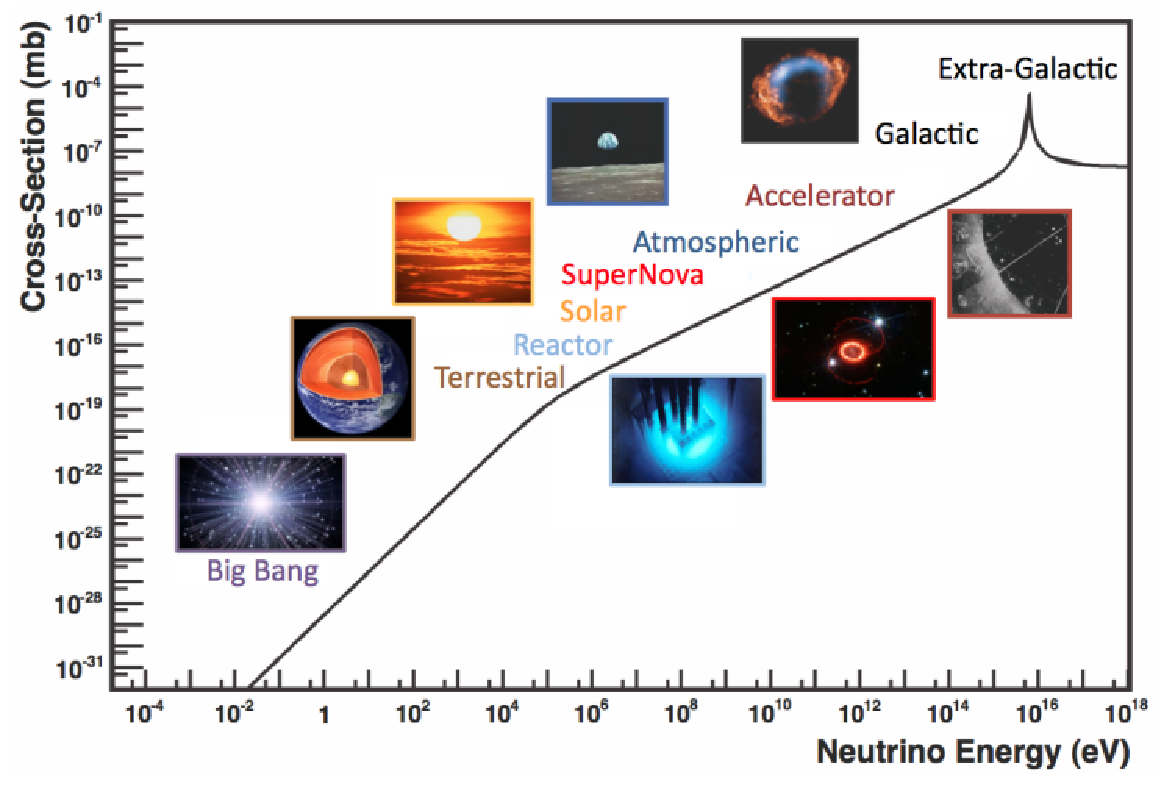
\includegraphics[width=\textwidth, trim={0mm 0mm 0mm 0mm}, clip,page=1]{Figures/Theory/EnergySpectrum.pdf}
  \end{subfigure}
  \caption{The electro-weak cross-section for \quickmath{\bar{\nu_{e}} + e^{-} \rightarrow \bar{\nu_{e}} + e^{-}} scattering on free electrons from various natural and man-made neutrino sources, as a function of neutrino energy. Taken from \cite{Formaggio:2012cpf}}
  \label{fig:NeutrinoOscillationPhysics_EnergySpectrum}
\end{figure}

\subsection{Solar Neutrinos}
\label{subsec:NeutrinoOscillationPhysics_SolarNeutrinos}

Solar neutrinos are emitted from fusion reaction chains at the centre of the Sun. The solar neutrino flux, given as a function of neutrino energy for different fusion and decay chains, is illustrated in \autoref{fig:NeutrinoOscillationPhysics_SolarNeutrinoFlux}. Whilst proton-proton fusion generates the largest flux of neutrinos, the neutrinos are low energy and are difficult to reconstruct due to the IBD interaction threshold of \quickmath{1.8\text{MeV}} \cite{Oralbaev_2016}. Consequently, most experiments focus on the neutrinos from the decay of \quickmath{^{8}B} (via \quickmath{^{8}B \rightarrow ^{8}Be^{*} + e^{+} + \nu_{e}}), which are higher energy.

\begin{figure}[h]
  \begin{subfigure}[t]{0.80\textwidth}
    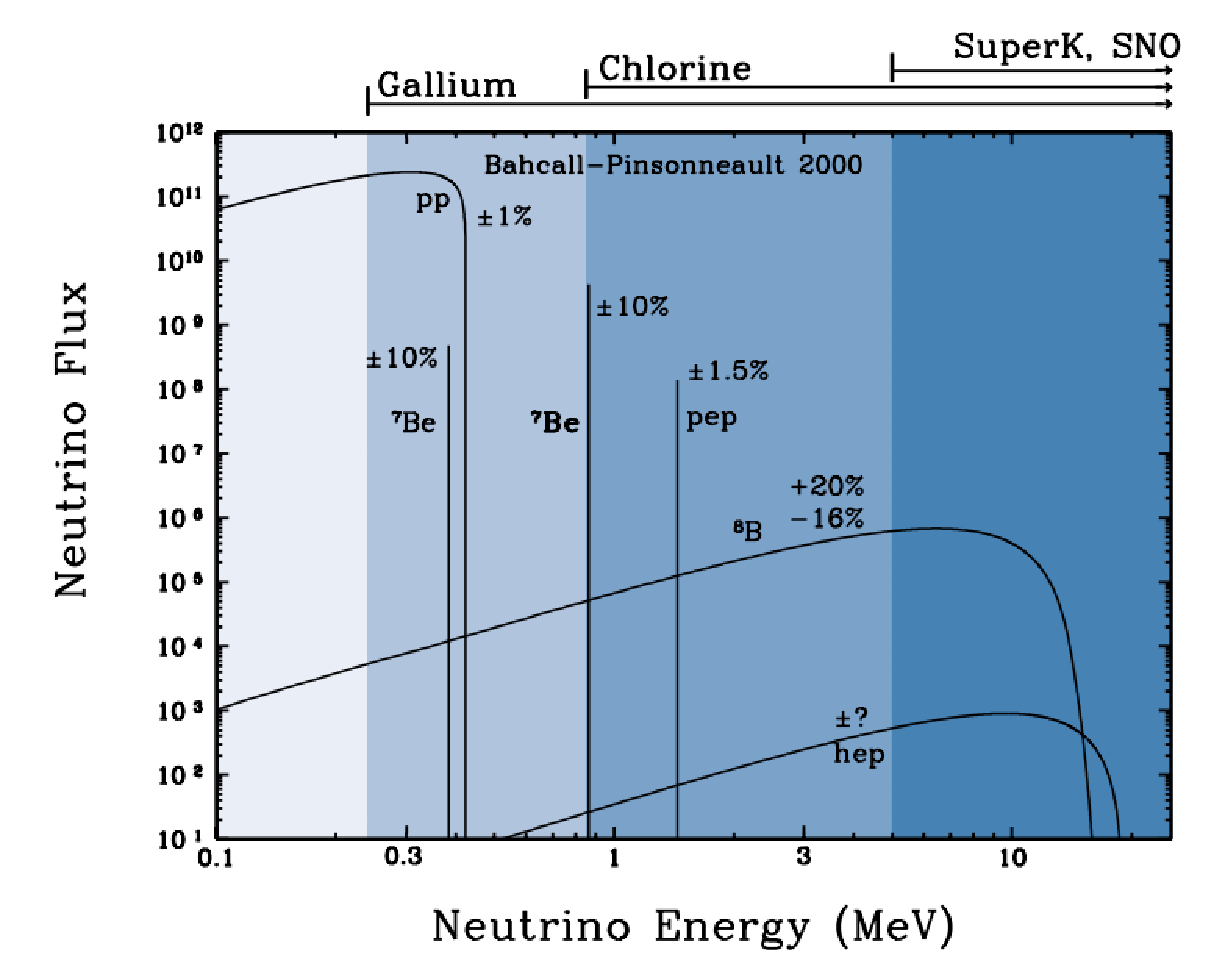
\includegraphics[width=\textwidth, trim={0mm 0mm 0mm 0mm}, clip,page=1]{Figures/Theory/SolarNeutrinoFlux.pdf}
  \end{subfigure}
  \caption{The solar neutrino flux as a function of neutrino energy for various fusion reactions and decay chains as predicted by the Standard Solar Model. Taken from \cite{Bellerive2004-ur}.}
  \label{fig:NeutrinoOscillationPhysics_SolarNeutrinoFlux}
\end{figure}

The first measurements of solar neutrinos observed a significant reduction in the event rate compared to predictions from the Standard Solar Model \cite{PhysRevLett.20.1205, Vinyoles2017-vv}. A proposed solution to this ``solar neutrino problem'' was \quickmath{\nu_{e} \leftrightarrow \nu_{\mu}} oscillations in a precursory version of the PMNS model \cite{Gribov1969-xi}. The Kamiokande \cite{PhysRevLett.63.16}, Gallex \cite{Hampel1999-of} and Sage \cite{PhysRevC.60.055801} experiments confirmed the \quickmath{\sim 0.5} factor deficit of solar neutrinos.

The conclusive solution to this problem was determined by the SNO collaboration \cite{Ahmad2002-zv}. Using a deuterium water target to observe \quickmath{^{8}B} neutrinos, the event rate of charged current (CC), neutral current (NC), and elastic scattering (ES) interactions (Given in \autoref{eq:NeutrinoOscillationPhysics_SNOInteractions}) was simultaneously measured. CC events can only occur for electron neutrinos, whereas the NC channel is agnostic to neutrino flavour, and the ES reaction has a small excess sensitivity for the detection of electron neutrino interactions. This meant that there were direct measurements of the \quickmath{\nu_{e}} and \quickmath{\nu_x} neutrino flux. It was concluded that the CC and ES interaction rates were consistent with the deficit previously observed. Most importantly, the NC reaction rate was only consistent with the others under the hypothesis of flavour transformation.

\begin{equation}
  \label{eq:NeutrinoOscillationPhysics_SNOInteractions}
  \begin{split}
    \nu_{e} + d &\rightarrow p + p + e^{-} \hspace{2cm} (CC) \\
    \nu_{x} + d &\rightarrow p + n + \nu_{x} \hspace{2.02cm} (NC) \\
    \nu_{x} + e^{-} &\rightarrow \nu_{x} + e^{-} \hspace{2.55cm} (ES)
  \end{split}
\end{equation}

Since the SNO measurement, many experiments have since measured the neutrino flux of different interaction chains within the sun \cite{Borexino_Collaboration2018-of, Aharmim2006-yb, Agostini2020-so}. The most recent measurement was that of CNO-cycle neutrinos which were recently observed with \quickmath{5\sigma} significance by the Borexino collaboration \cite{Borexino_Collaboration2018-of}.
%Future neutrino experiments aim to further these spectroscopic measurements of different fusion chains within the Sun \cite{Andringa2016-zd, Beacom2017-ff, An2016-gm}. %Solar neutrinos act as an irreducible background for dark matter experiments like DARWIN but oscillation parameter measurements can be made \cite{aalbers2020solar}.

\subsection{Accelerator Neutrinos}
\label{subsec:NeutrinoOscillationPhysics_AcceleratorNeutrinos}

The concept of using an artificial ``neutrino beam'' was first realised in 1962 \cite{Danby1962-ph}.
%and led to the first discovery that \quickmath{\nu_{e}} and \quickmath{\nu_{\mu}} were in fact different particles.
Since then, many experiments have adopted the same fundamental concepts. Typically, a proton beam is aimed at a target producing charged mesons that decay to neutrinos. The mesons can be sign-selected by the use of magnetic focusing horns to generate a neutrino or antineutrino beam.
%Absorbing material and the rock between the target and detector absorb all particles barring the neutrinos.
Pions are the primary mesons that decay and depending on the orientation of the magnetic field, a muon (anti-)neutrino beam is generated via \quickmath{\pi^{+} \rightarrow \mu^{+} + \nu_{\mu}} or \quickmath{\pi^{-} \rightarrow \mu^{-} + \bar{\nu}_{\mu}}. The decay of muons and kaons results in an irreducible intrinsic electron neutrino background. In T2K, this background contamination is \quickmath{O(<1\%)} \cite{Abe_2013}. There is also an approximately \quickmath{\sim 5\%} ``wrong-sign'' neutrino background of \quickmath{\bar{\nu}_{\mu}} generated via the same decays. As the beam is generated by proton interactions (rather than anti-proton interactions), the wrong-sign component in the antineutrino beam is larger when operating in neutrino mode.

Tuning the proton energy in the beam and using beam focusing techniques allows the neutrino energy to be set to a value that maximises the disappearance oscillation probability in the \quickmath{L/E} term in \autoref{eq:NeutrinoOscillationPhysics_PMNS_2FlavourOscProb}.
%As the inital proton beam can be tuned resulting in a tunable neutrino energy spectra, the advantage of these type of experiments is that they can be focused in on the oscillation dip presented by the \quickmath{L/E} term in \autoref{eq:NeutrinoOscillationPhysics_PMNS_2FlavourOscProb} using the two flavour approximation.
This means that accelerator experiments are typically more sensitive to the mixing parameters as compared to a natural neutrino source. However, the disadvantage compared to atmospheric neutrino experiments is the cost of building a facility to provide high-energy neutrinos, with a high flux, which is required for longer baselines. Consequently, there is typically less sensitivity to matter effects and the ordering of the neutrino mass eigenstates.

A neutrino experiment measures

\begin{equation}
  \label{eq:NeutrinoOscillationPhysics_DetectorMeasurement}
  R(\vec{x}) = \Phi(E_{\nu}) \times \sigma(E_{\nu}) \times \epsilon(\vec{x}) \times P(\nu_{\alpha} \rightarrow \nu_{\beta}),
\end{equation}

where \quickmath{R(\vec{x})} is the event rate of neutrinos at position \quickmath{\vec{x}}, \quickmath{\Phi(E_{\nu})} is the flux of neutrinos with energy \quickmath{E_{\nu}}, \quickmath{\sigma(E_{\nu})} is the cross-section of the neutrino interaction and \quickmath{\epsilon(\vec{x})} is the efficiency and resolution of the detector. In order to leverage the most out of an accelerator neutrino experiment, the flux and cross-section systematics need to be constrained. This is typically done via the use of a ``near detector'', situated at a baseline of \quickmath{O(1)\text{km}}. This detector observes the unoscillated neutrino flux and constrains the parameters used within the flux and cross-section model.

The first accelerator experiments to precisely measure oscillation parameters were MINOS \cite{PhysRevLett.97.191801} and K2K \cite{PhysRevLett.9.36}.
These experiments confirmed the \quickmath{\nu_{\mu}} disappearance seen in atmospheric neutrino experiments by finding consistent parameter values for \quickmath{\sin^{2}(\theta_{23})} and \quickmath{\Delta m^{2}_{32}}.
The current generation of accelerator neutrino experiments, T2K and \quickmath{\text{NO}\nu\text{A}} extended this field by observing \quickmath{\bar{\nu}_{\mu} \rightarrow \bar{\nu}_{e}} and lead the sensitivity to atmospheric mixing parameters as seen in \autoref{fig:NeutrinoOscillationPhysics_AtmosphericParamContour} \cite{PhysRevLett.123.151803}.
The two experiments differ in their peak neutrino energy, baseline, and detection technique.
The \quickmath{\text{NO}\nu\text{A}} experiment is situated at a baseline of \quickmath{810\text{km}} from the NuMI beamline which delivers \quickmath{2\text{GeV}} neutrinos.
The T2K neutrino beam is peaked around \quickmath{0.6 \text{GeV}} and propagates \quickmath{295\text{km}} \cite{t2k_det}.
Additionally, the \quickmath{\text{NO}\nu\text{A}} experiment uses functionally identical detectors (near and far) whereas T2K uses a plastic scintillator technique at the near detector and a water Cherenkov far detector.
The future generation experiments DUNE \cite{Abi2020-cm} and Hyper-Kamiokande \cite{Hyper-Kamiokande_Proto-Collaboration2015-ac} will succeed these experiments as the high-precision era of neutrino oscillation parameter measurements develops.

Several anomalous results have been observed in the LSND \cite{PhysRevD.64.112007} and MiniBooNE \cite{PhysRevLett.110.161801} detectors which were designed with purposefully short baselines. Parts of the neutrino community attributed these results to oscillations induced by a fourth ``sterile'' neutrino \cite{Blanco_2020} but several searches in other experiments, MicroBooNE \cite{10.48550/arxiv.2110.14054} and KARMEN \cite{PhysRevD.65.112001}, found no hints of additional neutrino species. The solution to the anomalous results is still being determined.

\subsection{Atmospheric Neutrinos}
\label{subsec:NeutrinoOscillationPhysics_AtmosphericNeutrinos}

The interactions of primary cosmic ray protons in the Earth's upper atmosphere generate showers of energetic hadrons. These are mostly pions and kaons that decay to produce a natural source of neutrinos spanning energies of MeV to TeV \cite{Gaisser2002-gl}. The main decay is via,

\begin{equation}
  \label{eq:NeutrinoOscillationPhysics_PionDecay}
  \begin{split}
    \pi^{\pm} &\rightarrow \mu^{\pm} + (\nu_{\mu},\bar{\nu}_\mu), \\
    \mu^{\pm} &\rightarrow e^{\pm} + (\nu_{\mu},\bar{\nu}_\mu) + (\nu_{e},\bar{\nu}_e),
  \end{split}
\end{equation}

such that for a single pion decay, three neutrinos can be produced. The atmospheric neutrino flux energy spectra as predicted by the Bartol \cite{Barr_2004}, Honda \cite{Honda_2007, PhysRevD.70.043008, Honda:2011}, and FLUKA \cite{etde_20239111} models are illustrated in \autoref{fig:NeutrinoOscillationPhysics_AtmosphericNeutrinoFlux}. The flux distribution peaks at an energy of \quickmath{O(10) \text{GeV}}. The uncertainties associated with these models are dominated by the hadronic production of kaon and pions as well as the primary cosmic flux. 

\begin{figure}[h]
  \begin{subfigure}[t]{0.80\textwidth}
    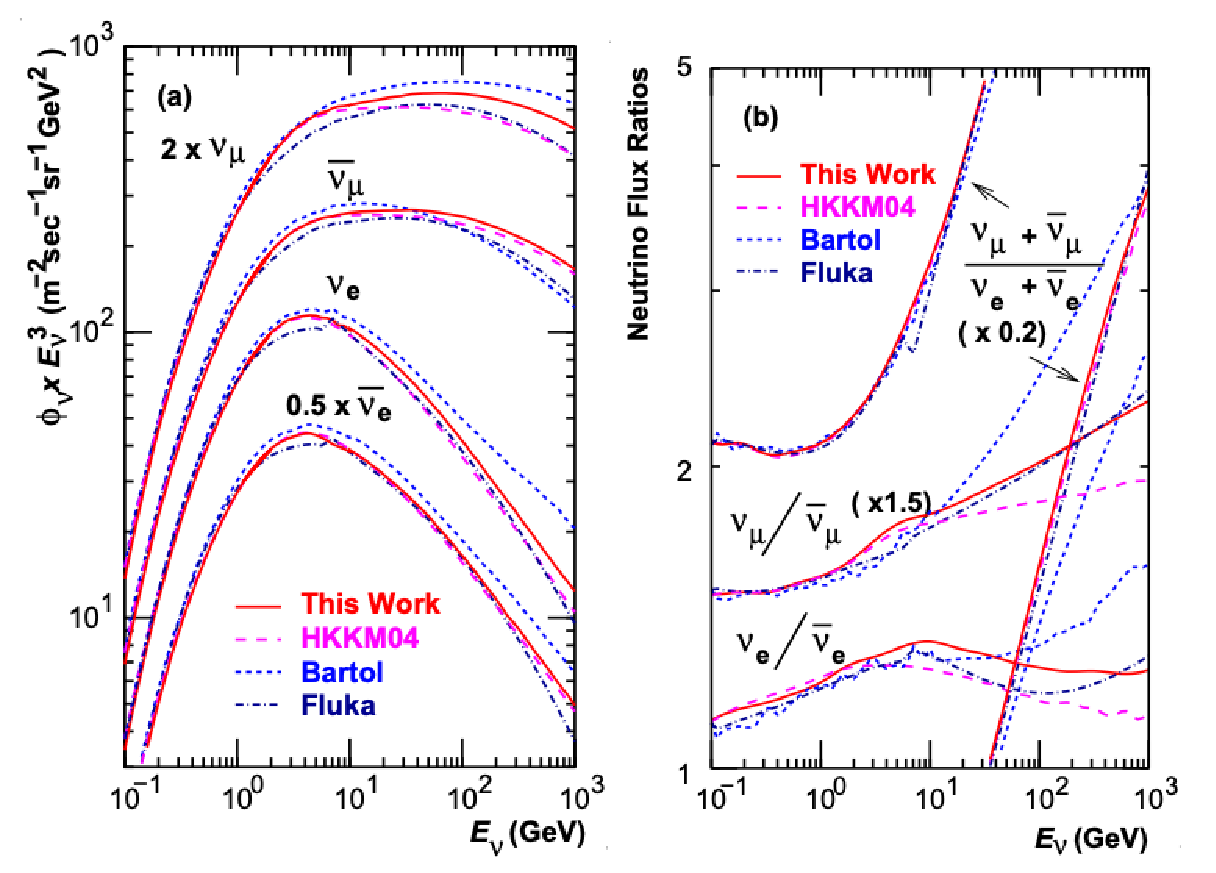
\includegraphics[width=\textwidth, trim={0mm 0mm 0mm 0mm}, clip,page=1]{Figures/Theory/AtmosphericNuFlux.pdf}
  \end{subfigure}
  \caption{Left panel: The atmospheric neutrino flux for different neutrino flavours as a function of neutrino energy as predicted by the 2007 Honda model (``This work'') \cite{Honda_2007}, the 2004 Honda model (``HKKM04'')\cite{PhysRevD.70.043008}, the Bartol model \cite{Barr_2004} and the FLUKA model \cite{etde_20239111}. Right panel: The ratio of the muon to electron neutrino flux as predicted by all the quoted models. Both figures taken from \cite{Honda_2007}.}
  \label{fig:NeutrinoOscillationPhysics_AtmosphericNeutrinoFlux}
\end{figure}

Unlike long-baseline experiments which have a fixed baseline, the distance atmospheric neutrinos propagate is dependent upon the zenith angle at which they interact. This is illustrated in \autoref{fig:NeutrinoOscillationPhysics_ZenithAngle}. Neutrinos that are generated directly above the detector (\quickmath{\cos(\theta)=1.0}) have a baseline equivalent to the height of the atmosphere, whereas neutrinos that interact directly below the detector (\quickmath{\cos(\theta)=-1.0}) have to travel a length equal to the diameter of the  Earth. This means atmospheric neutrinos have a baseline that varies from \quickmath{O(20)\text{km}} to \quickmath{O(6 \times 10^{3})\text{km}}. Any neutrino generated at or below the horizon will be subject to MSW matter resonance as they propagate through the Earth.

\begin{figure}[h]
  \begin{subfigure}[t]{0.40\textwidth}
    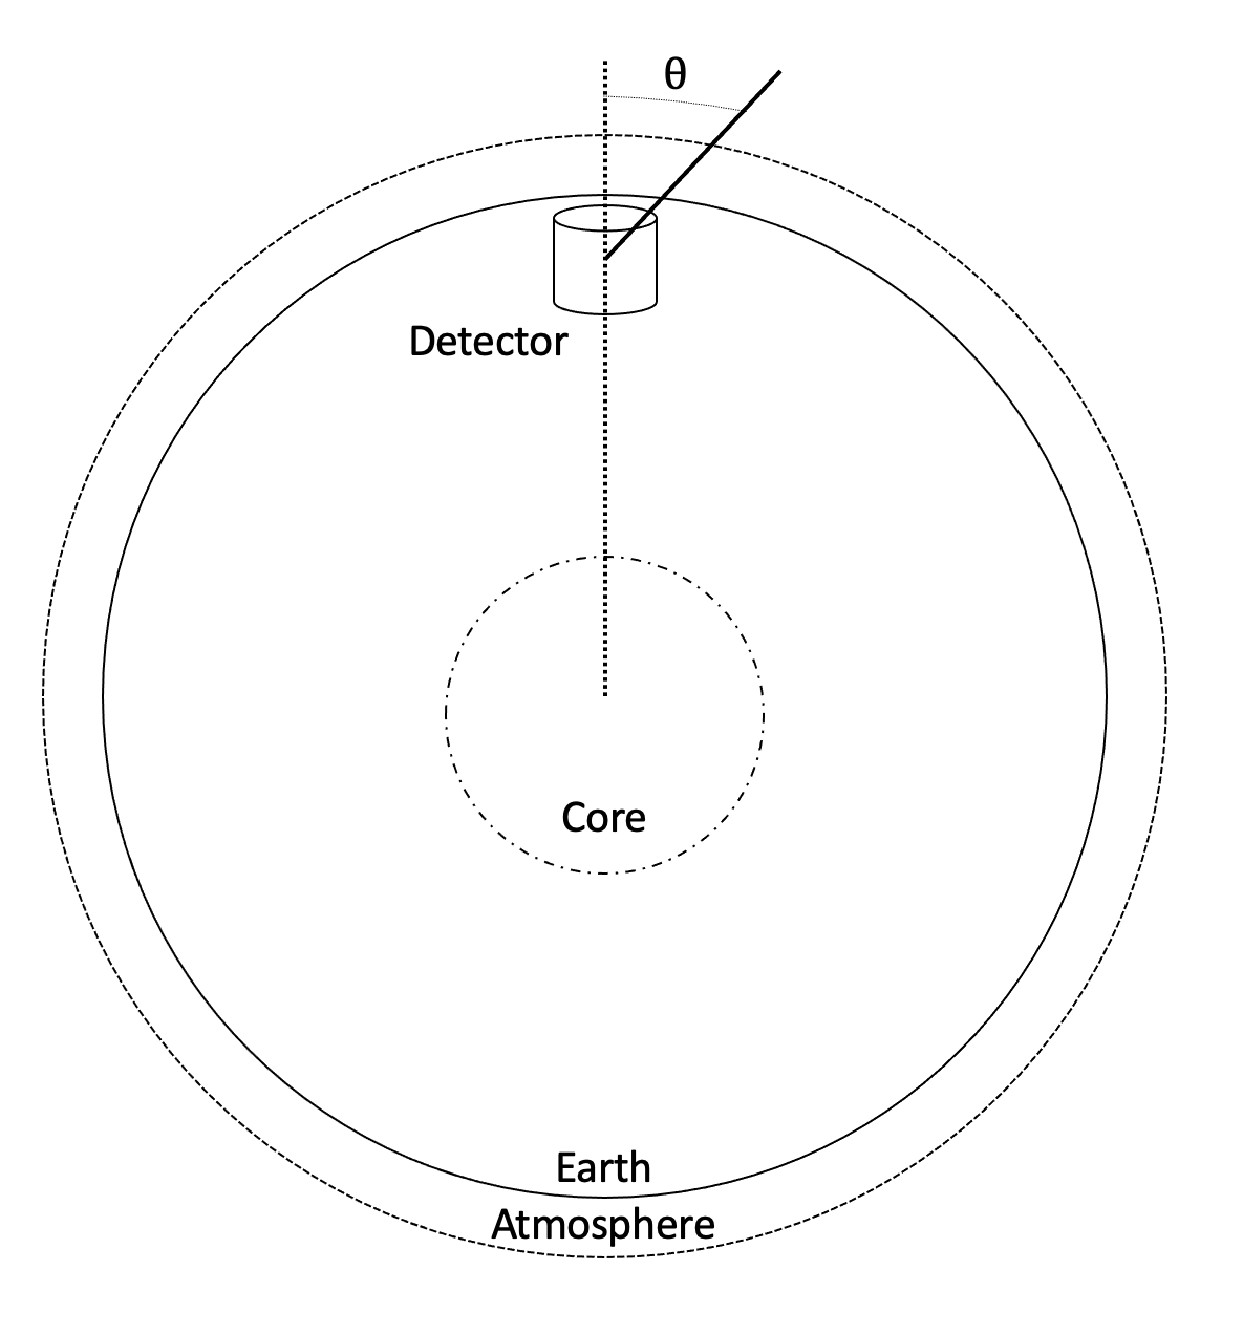
\includegraphics[width=\textwidth, trim={0mm 0mm 0mm 0mm}, clip,page=1]{Figures/Theory/ZenithAngle.pdf}
  \end{subfigure}
  \caption{A diagram illustrating the definition of zenith angle as used in the Super Kamiokande experiment \cite{Ashie_2005}.}
  \label{fig:NeutrinoOscillationPhysics_ZenithAngle}
\end{figure}

\autoref{fig:NeutrinoOscillationPhysics_NuFluxZenithAngleDep} highlights the neutrino flux as a function of the zenith angle for different slices of neutrino energy. For medium to high-energy neutrinos (and to a lesser degree for low-energy neutrinos), the flux is approximately symmetric around \quickmath{\cos(\theta)=0}. To the accuracy of this approximation, the systematic uncertainties associated with atmospheric flux for comparing upward-going and down-going neutrino cancels. This allows the down-going events, which are mostly insensitive to oscillation probabilities, to act as an unoscillated prediction (similar to a near detector in an accelerator neutrino experiment).

\begin{figure}[h]
  \begin{subfigure}[t]{0.90\textwidth}
    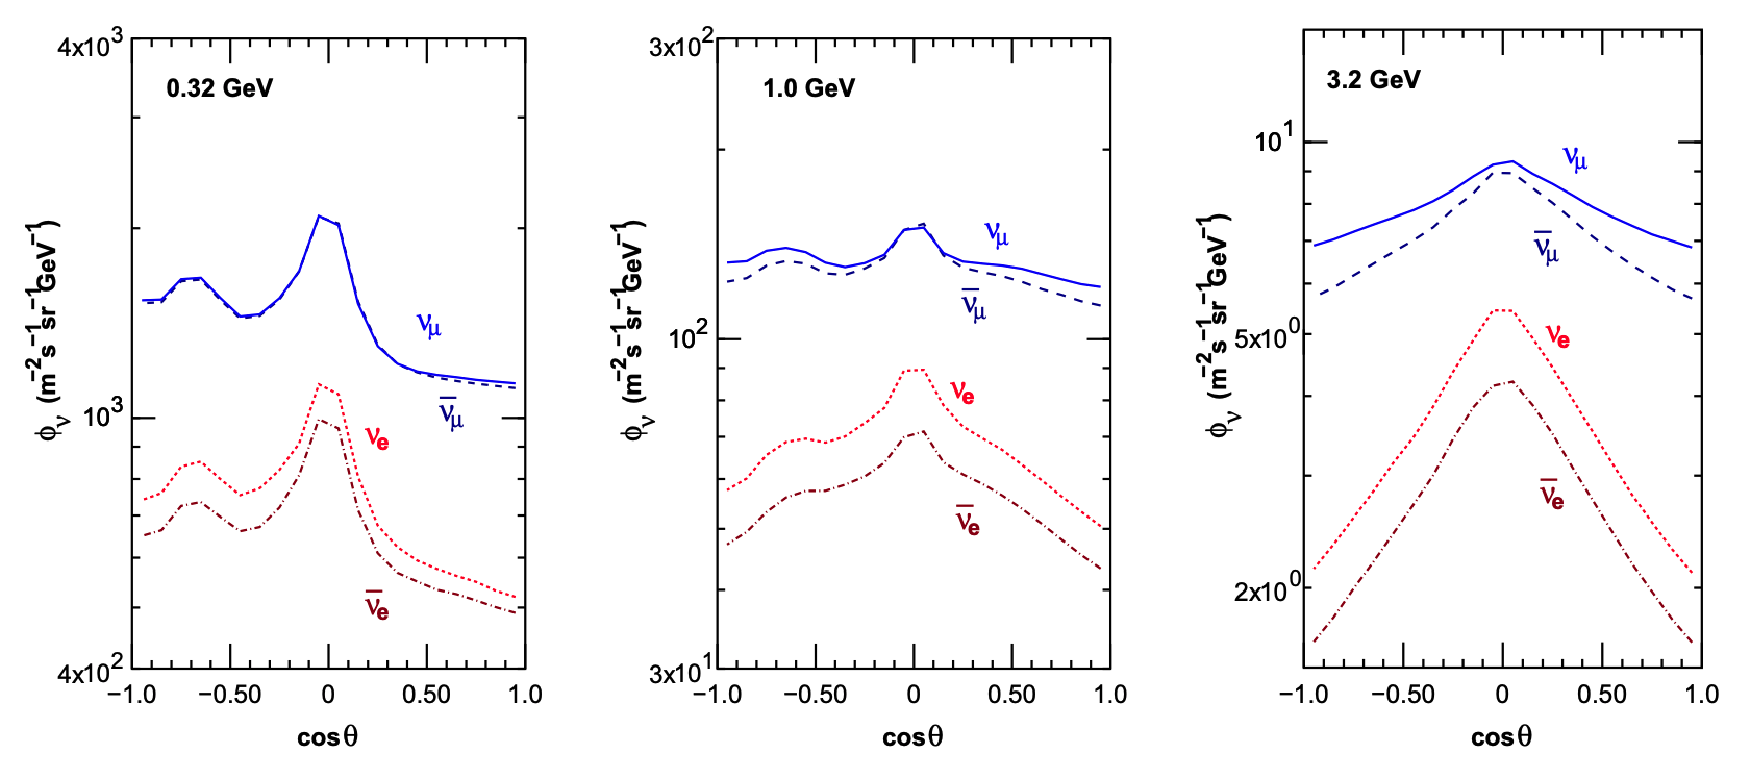
\includegraphics[width=\textwidth, trim={0mm 0mm 0mm 0mm}, clip,page=1]{Figures/Theory/NuFluxZenithAngleDep.pdf}
  \end{subfigure}
  \caption{Prediction of \quickmath{\nu_e, \bar{\nu}_{e}, \nu_{\mu}, \bar{\nu}_{\mu}} fluxes as a function of zenith angle as calculated by the HKKM model \cite{Honda:2011}. The left, middle and right panels represent three values of neutrino energy, \quickmath{0.32\text{GeV}}, \quickmath{1.0\text{GeV}} and \quickmath{3.2\text{GeV}} respectively. Predictions for other models including Bartol \cite{Barr_2004}, Honda \cite{Honda_2007} and FLUKA \cite{etde_20239111} are given in \cite{Ashie_2005}.}
  \label{fig:NeutrinoOscillationPhysics_NuFluxZenithAngleDep}
\end{figure}

Precursory hints of atmospheric neutrinos were observed in the mid-1960s searching for \quickmath{\overset{(-)}{\nu_\mu} + X \rightarrow X^{*} + \mu^{\pm}} \cite{Reines1965-cf}.
%, although it was called an anomaly at the time of measurement.
This was succeeded by the IMB-3 \cite{PhysRevLett.66.2561} and Kamiokande \cite{Hirata1992-qz} experiments which measured the double ratio of muon to electron neutrinos in data to Monte Carlo, \quickmath{R(\nu_{\mu}/\nu_{e}) = (\mu/e)_{Data}/(\mu/e)_{MC}}. Both experiments were found to have a consistent deficit of muon neutrinos, with \quickmath{R(\nu_{\mu}/\nu_{e}) = 0.67 \pm 0.17} and \quickmath{R(\nu_{\mu}/\nu_{e}) = 0.658 \pm 0.016 \pm 0.035}, respectively. %Soudan-2 \cite{Allison1997-qz} determined similar measurements.
Super-Kamiokande (SK) \cite{Ashie_2005} extended this analysis by fitting oscillation parameters in \quickmath{P(\nu_\mu \rightarrow \nu_\tau)} which found best fit parameters \quickmath{\sin^{2}(2\theta) > 0.92} and \quickmath{1.5 \times 10^{-3} < \Delta m^{2} < 3.4 \times 10^{-3} \text{eV}^{2}}.

Since then, atmospheric neutrino experiments have been making precision measurements of the \quickmath{\sin^{2}(\theta_{23})} and \quickmath{\Delta m^{2}_{32}} oscillation parameters.
%, and to a lesser extent the sign of \quickmath{\Delta m^{2}_{32}} through the matter resonance present for any neutrinos passing through the Earth.
Atmospheric neutrino oscillation is dominated by \quickmath{P(\nu_{\mu} \rightarrow \nu_{\tau})}, where SK observed a \quickmath{4.6\sigma} discovery of \quickmath{\nu_{\tau}} appearance \cite{Li_2018}. \autoref{fig:NeutrinoOscillationPhysics_AtmosphericParamContour} illustrates the current estimates on the atmospheric mixing parameters, from a wide range of atmospheric and accelerator neutrino observatories.

\begin{figure}[h]
  \begin{subfigure}[t]{0.90\textwidth}
    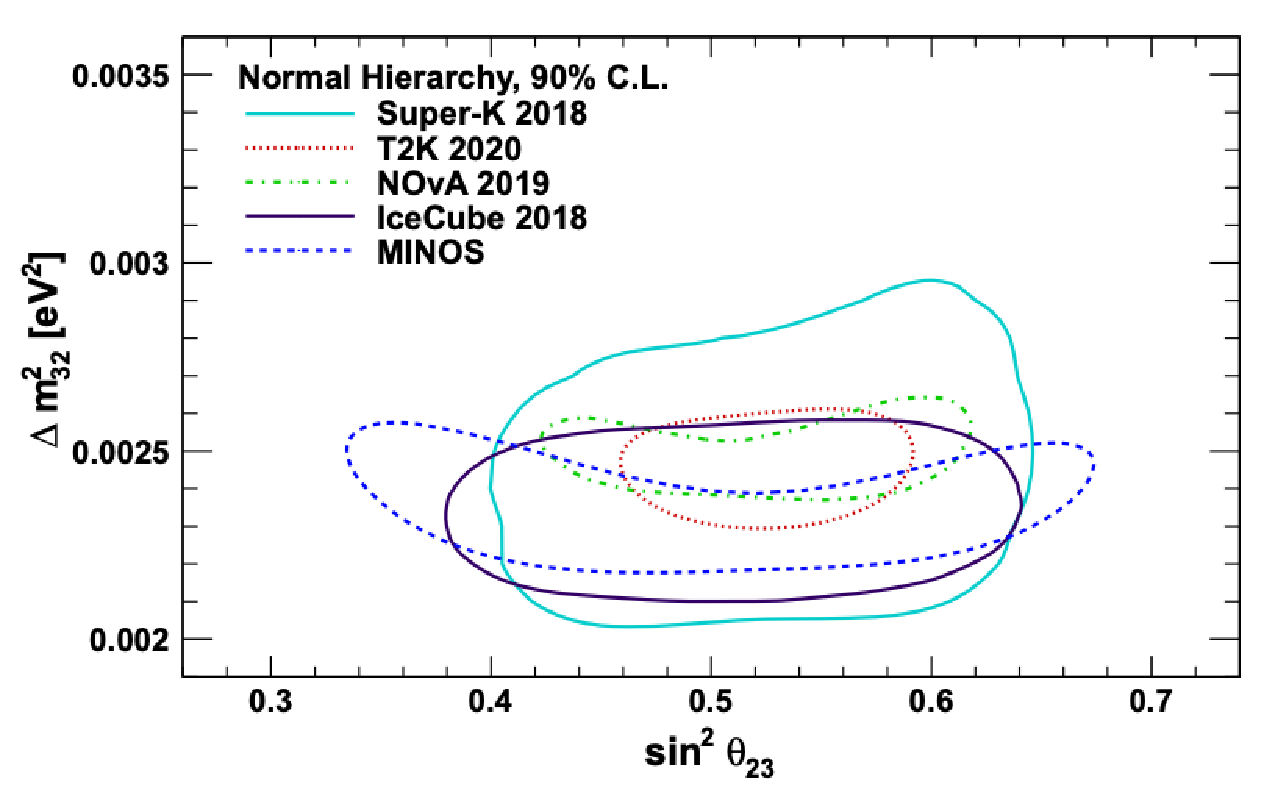
\includegraphics[width=\textwidth, trim={0mm 0mm 0mm 0mm}, clip,page=1]{Figures/Theory/AtmosphericParams.pdf}
  \end{subfigure}
  \caption{Constraints on the atmospheric oscillation parameters, \quickmath{\sin^{2}(\theta_{23})} and \quickmath{\Delta m^{2}_{32}}, from atmospheric and long-baseline experiments: SK \cite{Kamiokande_Collaboration2017-nf}, T2K \cite{T2K_Collaboration2018-sm}, \quickmath{\text{NO}\nu\text{A}} \cite{Acero2019-rw}, IceCube \cite{Aartsen2018-cz} and MINOS \cite{Adamson2014-tt}. Figure taken from \cite{Athar_2022}.}
  \label{fig:NeutrinoOscillationPhysics_AtmosphericParamContour}
\end{figure}

\subsection{Reactor Neutrinos}
\label{subsec:NeutrinoOscillationPhysics_ReactorNeutrinos}

As illustrated in the first discovery of neutrinos (\autoref{sec:NeutrinoOscillationPhysics_Discovery}), nuclear reactors are a very useful artificial source of electron antineutrinos. For reactors that use low-enriched uranium \quickmath{^{235}\text{U}} as fuel, the antineutrino flux is dominated by the \quickmath{\beta}-decay fission of \quickmath{^{235}\text{U}}, \quickmath{^{238}\text{U}}, \quickmath{^{239}\text{Pu}} and \quickmath{^{241}\text{Pu}} \cite{Kim2013-ye} as illustrated in \autoref{fig:NeutrinoOscillationPhysics_ReactorNeutrinoProduction}.

\begin{figure}[h]
  \begin{subfigure}[t]{0.90\textwidth}
    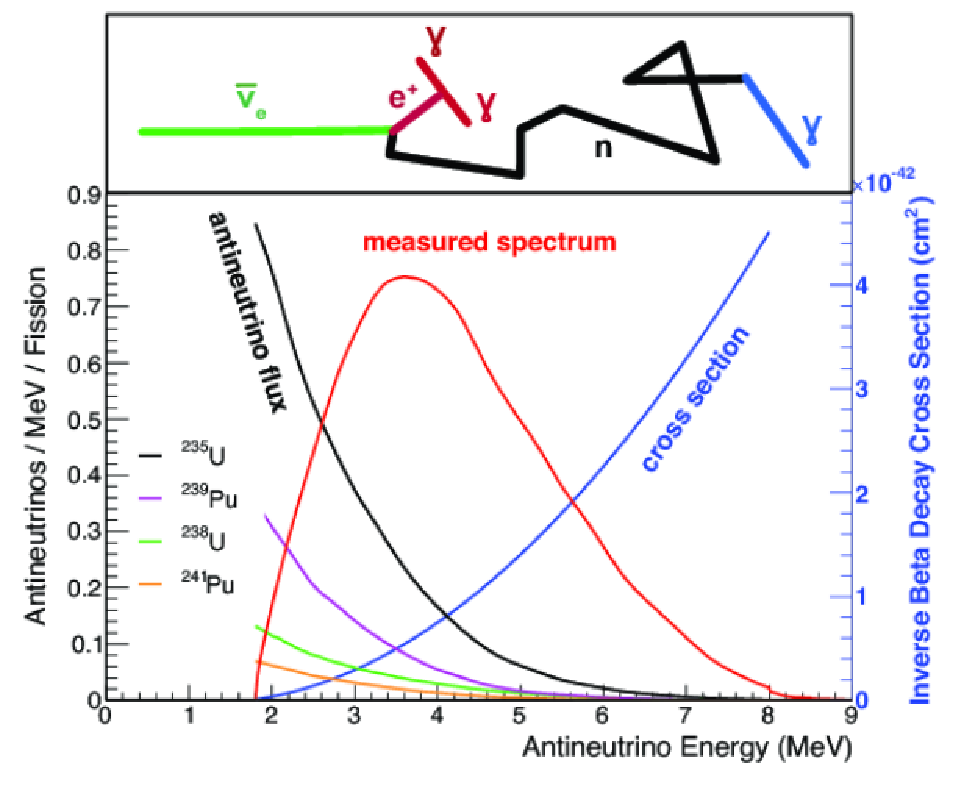
\includegraphics[width=\textwidth, trim={0mm 0mm 0mm 0mm}, clip,page=1]{Figures/Theory/ReactorNeutrinoProduction.pdf}
  \end{subfigure}
  \caption{Reactor electron antineutrino fluxes for \quickmath{^{235}\text{U}} (Black), \quickmath{^{238}\text{U}} (Green), \quickmath{^{239}\text{Pu}} (Purple), and \quickmath{^{241}\text{Pu}} (Orange) isotopes. The inverse \quickmath{\beta}-decay cross-section (Blue) and corresponding measurable neutrino spectrum (Red) are also given. Top panel: Schematic of Inverse \quickmath{\beta}-decay interaction including the eventual capture of the emitted neutron. This capture emits a \quickmath{\gamma}-ray which provides a second signal of the event. Taken from \cite{SajjadAthar:2021prg}.}
  \label{fig:NeutrinoOscillationPhysics_ReactorNeutrinoProduction}
\end{figure}

Due to their low energy, reactor electron antineutrinos predominantly interact via the inverse \quickmath{\beta}-decay (IBD) interaction. The typical signature contains two signals delayed by \quickmath{O(200)\mu\text{s}}; firstly the prompt photons from positron annihilation, and secondly the photon emitted (\quickmath{E_{tot}^{\gamma} = 2.2\text{MeV}}) from de-excitation after neutron capture on hydrogen. Searching for both signals improves the detector's ability to distinguish between background and signal events \cite{Abe2022-ij}. %Recently, SK included gadolinium dopants into the ultra-pure water to increase the energy released from the photon cascade to \quickmath{\sim 8\text{MeV}} and reduce the time of the delayed signal to \quickmath{\sim 28 \mu \text{s}}.

There are many short baseline experiments (\quickmath{\text{L} \sim O(1)\text{km}}) that have measured the \quickmath{\sin^{2}(\theta_{13})} and \quickmath{\Delta m^{2}_{32}} oscillation parameters. Daya Bay \cite{PhysRevLett.108.171803}, RENO \cite{PhysRevLett.108.191802} and Double Chooz \cite{PhysRevLett.108.131801} have all provided precise measurements, with the first discovery of a non-zero \quickmath{\theta_{13}} made by Daya Bay and RENO (and complemented by T2K \cite{PhysRevLett.108.131801}). The constraints on \quickmath{\sin^{2}(\theta_{13})} by the reactor experiments lead the field. They are often used as external inputs to accelerator neutrino experiments to improve their sensitivity to \quickmath{\delta_{CP}} and mass hierarchy determination.
%One curiosity of these short baseline reactor experiments is the `\quickmath{5 \text{MeV}} excess' \cite{Berryman_2019}. First observed in 2014 \cite{For_the_RENO_Collaboration2015-zy, Abe_2014}, all three experiments listed observed a shape excess in events around \quickmath{E_{\nu} \sim 5 \text{MeV}}. The reason behind this excess is speculated to be either oscillations to sterile neutrinos or a fault in the Huber-Mueller model \cite{Mueller_2011}. At this time, the latter is favoured as Daya Bay \cite{PhysRevLett.123.111801} observed substantial evidence (\quickmath{4.0\sigma}) of correlation between the excess and the \quickmath{^{235}\text{U}} electron antineutrino flux.
%Other neutrino experiments, PROSPECT \cite{PhysRevD.103.032001} and STEREO \cite{STEREO} show similar results data to help determine the cause of the excess.
JUNO-TAO \cite{junocollaboration2020tao}, a small collaboration within the larger JUNO experiment, is a next-generation reactor experiment that aims to precisely measure the isotopic antineutrino yields from the different fission chains. %Alongside this, it aims to explain the `\quickmath{5 \text{MeV}} excess' of neutrino events observed by other reactor neutrino experiments \cite{For_the_RENO_Collaboration2015-zy, Abe_2014, PhysRevLett.123.111801}. It does this by conducting a search for sterile neutrinos with a mass scale of around \quickmath{1 \text{eV}}.

Kamland \cite{Decowski2016-hh} is the only experiment to have observed reactor neutrinos using a long baseline (flux weighted averaged baseline of \quickmath{L \sim 180\text{km}}) which allows it to have sensitivity to \quickmath{\Delta m^{2}_{21}}. Combined with the SK solar neutrino experiment, the combined analysis puts the most stringent constraint on \quickmath{\Delta m^{2}_{21}} \cite{PhysRevD.83.052002}.

\section{Summary Of Oscillation Parameter Measurements}
\label{sec:Theory_Summary}

Since the first evidence of neutrino oscillations, numerous measurements of the mixing parameters have been made. Many experiments use neutrinos as a tool for the discovery of new physics (diffuse supernova background, neutrinoless double beta decay and others) so the PMNS parameters are summarised in the Particle Data Group (PDG) review tables. The analysis presented in this thesis focuses on the 2020 T2K oscillation analysis presented in \cite{Dunne2020-uf} which the 2020 PDG constraints \cite{Particle_Data_Group2020-ms} were used. These constraints are outlined in \autoref{tab:Theory_PDGConstraints}.

\begin{table}[ht!]
    \centering
    \begin{tabular}{c|c}
      \hline
      Parameter & 2020 Constraint \\
      \hline
      \quickmath{\sin^{2}(\theta_{12})} & \quickmath{0.307 \pm 0.013} \\
      \quickmath{\Delta m^{2}_{21}} & \quickmath{(7.53 \pm 0.18) \times 10^{-5} \text{eV}^{2}} \\
      \quickmath{\sin^{2}(\theta_{13})} & \quickmath{(2.18 \pm 0.07) \times 10^{-2}} \\
      \quickmath{\sin^{2}(\theta_{23})} (I.H.) & \quickmath{0.547 \pm 0.021} \\
      \quickmath{\sin^{2}(\theta_{23})} (N.H.) & \quickmath{0.545 \pm 0.021} \\
      \quickmath{\Delta m^{2}_{32}} (I.H.) & \quickmath{(-2.546^{+0.034}_{-0.040}) \times 10^{-3} \text{eV}^{2}} \\
      \quickmath{\Delta m^{2}_{32}} (N.H.) & \quickmath{(2.453\pm0.034) \times 10^{-3} \text{eV}^{2}} \\
      \hline
      \hline
    \end{tabular}
    \caption{The 2020 Particle Data Group constraints of the oscillation parameters taken from \cite{Particle_Data_Group2020-ms}. The value of \quickmath{\Delta m^{2}_{32}} is given for both normal hierarchy (N.H.) and inverted hierarchy (I.H.) and \quickmath{\sin^{2}(\theta_{23})} is broken down by whether its value is below (Q1) or above (Q2) \quickmath{0.5}.}
    \label{tab:Theory_PDGConstraints}
\end{table}

The \quickmath{\sin^{2}(\theta_{13})} measurement stems from the electron antineutrino disappearance, \quickmath{P(\bar{\nu}_{e} \rightarrow \bar{\nu}_{e})}, and is taken as the  average best-fit from the combination of Daya Bay, Reno and Double Chooz. It is often used as a prior uncertainty within other neutrino oscillation experiments, typically termed the reactor constraint. The \quickmath{\sin^{2}(\theta_{12})} parameter is predominantly measured through electron neutrino disappearance, \quickmath{P(\nu_{e} \rightarrow \nu_{\mu,\tau})}, in solar neutrino experiments. The long-baseline reactor neutrino experiment Kamland also has a sensitivity to this parameter and is used in a joint fit to solar data from SNO and SK, using the reactor constraint. Measurements of \quickmath{\sin^{2}(\theta_{23})} are made by long-baseline and atmospheric neutrino experiments. The PDG value is a joint fit of T2K, \quickmath{\text{NO}\nu\text{A}}, MINOS and IceCube DeepCore experiments. The latest T2K-only measurement, provided at Neutrino2020 and is the basis of this thesis, is given as \quickmath{\sin^{2}(\theta_{23}) = 0.546^{+0.024}_{-0.046}} \cite{Dunne2020-uf}. The PDG constraint on \quickmath{\Delta m^{2}_{21}} is provided by the KamLAND experiment using solar and geoneutrino data. This measurement utilised a \quickmath{\sin^{2}(\theta_{13})} constraint from accelerator (T2K, MINOS) and reactor neutrino (Daya Bay, RENO, Double Chooz) experiments. Accelerator measurements make some of the most stringent constraints on \quickmath{\Delta m^{2}_{32}} although atmospheric experiments have more sensitivity to the mass hierarchy determination. The PDG performs a joint fit of accelerator and atmospheric data, in both normal and inverted hierarchies separately. The latest T2K-only result is \quickmath{\Delta m^{2}_{32} = 2.49^{+0.058}_{-0.082} \times 10^{-3}\text{eV}^{2}} favouring normal hierarchy \cite{Dunne2020-uf}. The value of \quickmath{\delta_{CP}} is largely undetermined. CP-conserving values of \quickmath{0} and \quickmath{\pi} were rejected with \quickmath{\sim 2\sigma} intervals, as published in Nature, although more recent analyses have reduced the credible intervals to \quickmath{90\%}. Since the 2020 PDG publication, there has been a new measurement of \quickmath{\sin^{2}(\theta_{13}) = (2.20 \pm 0.07) \times 10^{-2}} \cite{Workman:2022ynf}, alongside updated \quickmath{\Delta m^{2}_{32}} and \quickmath{\sin^{2}(\theta_{23})} measurements.

Throughout this thesis, several sample spectra predictions and contours are presented, which require oscillation parameters to be assumed. \autoref{tab:Theory_ParameterSets} defines two sets of oscillation parameters, with ``Asimov A'' set being close to the preferred values from a previous T2K-only fit \cite{PhysRevLett.112.181801} and ``Asimov B'' being CP-conserving and further from maximal \quickmath{\theta_{23}} mixing.

\begin{table}[ht!]
    \centering
    \begin{tabular}{c|c|c}
      \hline
      \hline
      Parameter & Asimov A & Asimov B \\
      \hline
      \quickmath{\Delta m^{2}_{12}} & \multicolumn{2}{c}{\quickmath{7.53 \times 10^{-5} \text{eV}^{2}}} \\ \hline
      \quickmath{\Delta m^{2}_{32}} & \multicolumn{2}{c}{\quickmath{2.509 \times 10^{-3} \text{eV}^{2}}} \\ \hline
      \quickmath{\sin^{2}\left(\theta_{12}\right)} & \multicolumn{2}{c}{\quickmath{0.304}} \\ \hline
      \quickmath{\sin^{2}\left(\theta_{13}\right)} & \multicolumn{2}{c}{\quickmath{0.0219}} \\ \hline
      \quickmath{\sin^{2}\left(\theta_{23}\right)} & \quickmath{0.528} & \quickmath{0.45} \\ \hline
      \quickmath{\delta_{CP}} & \quickmath{-1.601} & \quickmath{0.0} \\ \hline
      \hline
    \end{tabular}
    \caption{Reference values of the neutrino oscillation parameters for two different oscillation parameter sets.}
    \label{tab:Theory_ParameterSets}
\end{table}

\section{Overview of Oscillation Effects}
\label{sec:Oscillation_Overview}

The analysis presented within this thesis focuses on the determination of oscillation parameters from atmospheric and beam neutrinos. Whilst subject to the same oscillation formalism, the way in which the two samples have sensitivity to the different oscillation parameters differs significantly.

Atmospheric neutrinos have a varying baseline, or ``path length'' \quickmath{L}, such that the distance each neutrino travels before interacting is dependent upon the zenith angle, \quickmath{\theta_{Z}}. As primary cosmic rays can interact anywhere between the Earth's surface and \quickmath{\sim50\text{km}} above that, the height, \quickmath{h}, in the atmosphere at which the neutrino was generated also affects the path length,

\begin{equation}
  L = \sqrt{\left(R_{E} + h\right)^{2} - R_{E}^{2} \left(1 - \cos^{2} \left(\theta_{Z} \right) \right)} - R_{E}\cos(\theta_{Z}).
\end{equation}

Where \quickmath{R_{E} = 6,371\text{km}} is the Earth's radius. This assumes a spherically symmetric Earth model. Therefore, the oscillation probability is dependent upon two parameters, \quickmath{\cos(\theta_{Z})} and \quickmath{E_{\nu}}.

The oscillation probability used within this analysis is based on \cite{Barger:1980tf}. The neutrino wavefunction in the vacuum Hamiltonian evolves in each layer of constant matter density via

\begin{equation}
  i \frac{d\psi_{j}(t)}{dt} = \frac{m_{j}^{2}}{2E_{\nu}} \psi_{j}(t) - \sum_{k} \sqrt{2} G_{F} N_{e} U_{ej} U_{ke}^{\dagger} \psi_{k}(t),
\end{equation}

where \quickmath{m_{j}^{2}} is the square of the \quickmath{j^{th}} vacuum eigenstate mass, \quickmath{E_{\nu}} is the neutrino energy, \quickmath{G_{F}} is Fermi's constant, \quickmath{N_{e}} is the electron number density and \quickmath{U} is the PMNS matrix. The transformation \quickmath{N_{e} \rightarrow -N_{e}} and \quickmath{\delta_{CP} \rightarrow -\delta_{CP}} is applied for antineutrino propagation. Thus, a model of the Earth's density is required for neutrino propagation. Following the official SK-only methodology \cite{thesis_roger}, this analysis uses the Preliminary Reference Earth Model (PREM) \cite{Dziewonski1981-sp} which provides piecewise cubic polynomials as a function of the Earth's radius. This density profile is illustrated in \autoref{fig:Oscillation_SK_PREMModelApproximation}. As the propagator requires layers of constant density, the SK methodology approximates the PREM model by using four layers of constant density \cite{thesis_roger}, detailed in \autoref{tab:NeutrinoOscillationPhysics_PREMModel}.

\begin{figure}[h]
  \begin{subfigure}[t]{0.8\textwidth}
    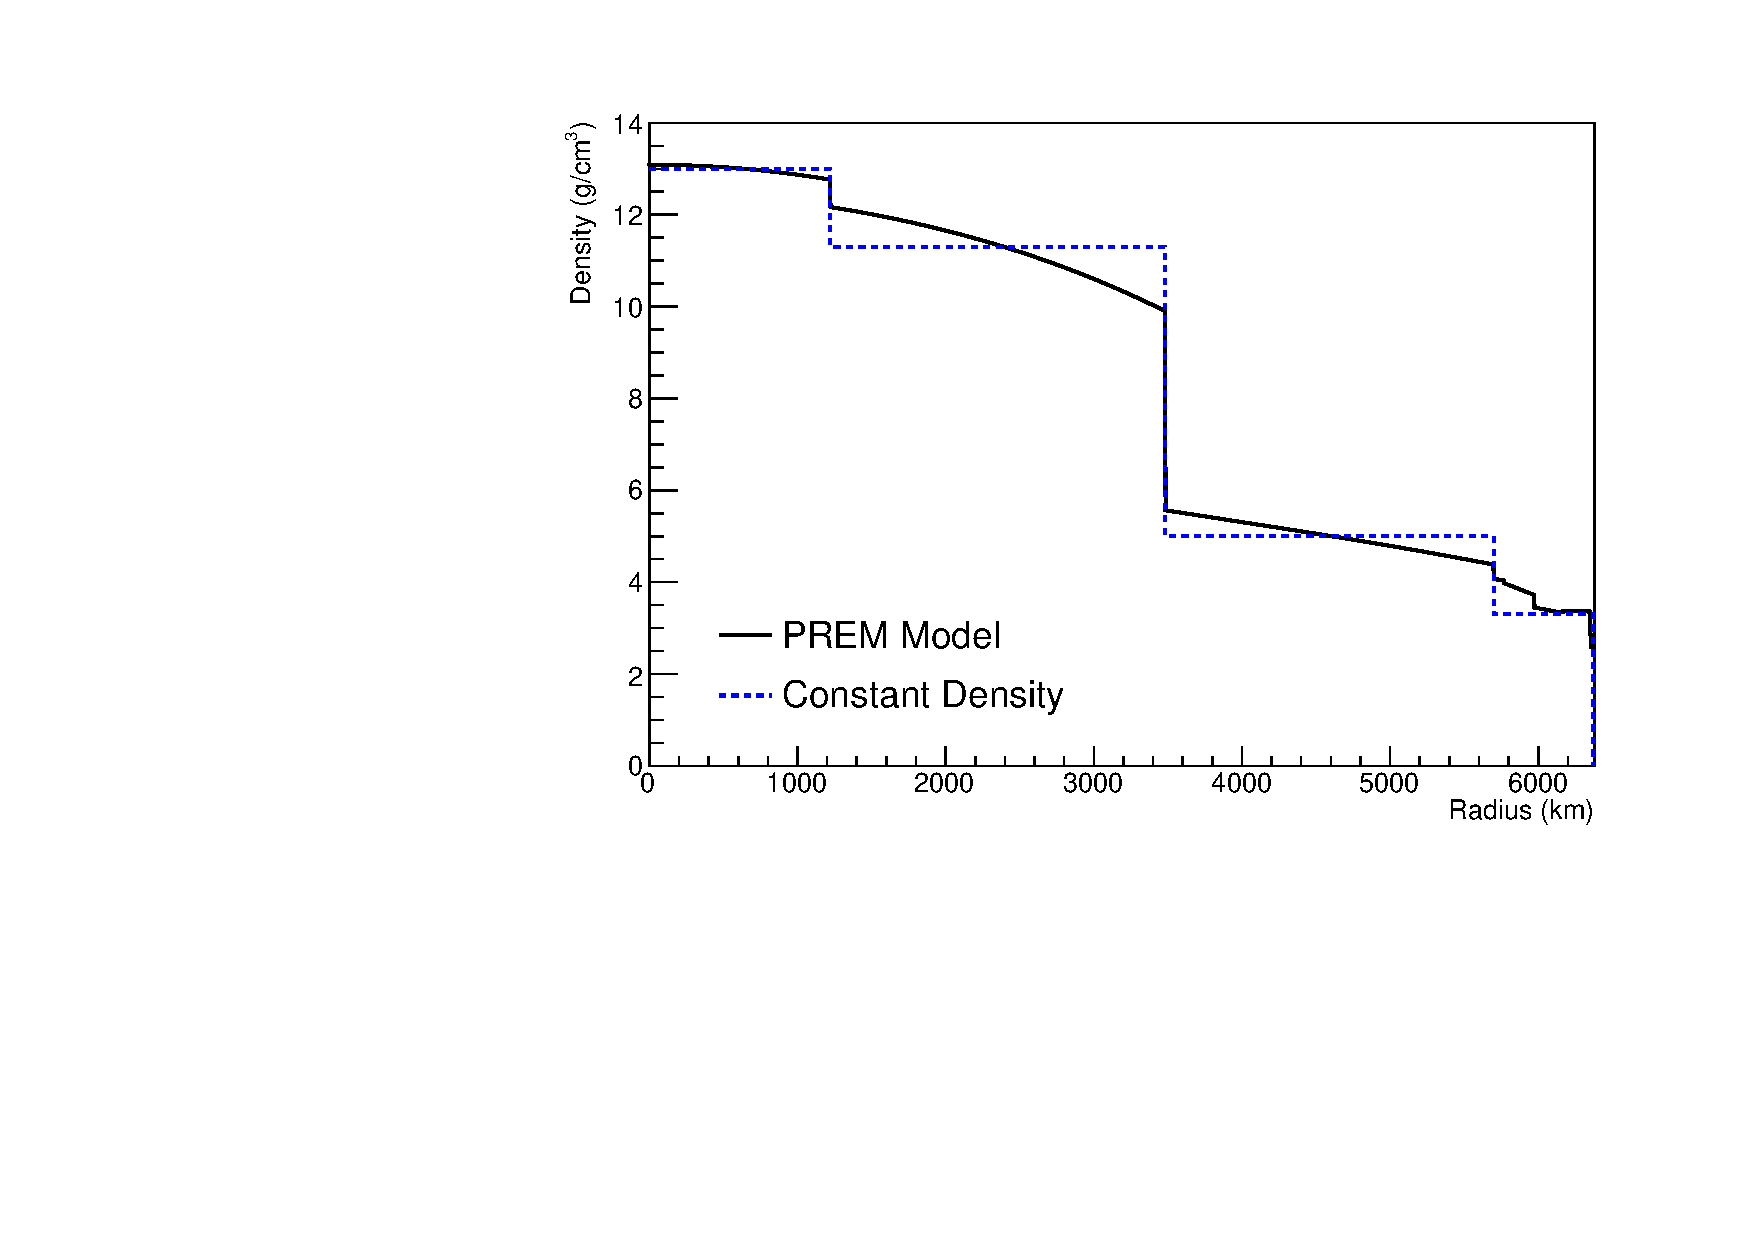
\includegraphics[width=\textwidth, trim={0mm 0mm 0mm 0mm}, clip,page=1]{Figures/Oscillation/DensityComparison.pdf}
  \end{subfigure}
  \caption{The density of the Earth given as a function of the radius, as given by the PREM model (Black), and the constant density four-layer approximation (Blue), as used in the official SK-only analysis.}
  \label{fig:Oscillation_SK_PREMModelApproximation}
\end{figure}

\begin{table}[ht!]
    \centering
    \begin{tabular}{c|c|c|c}
      \hline
      Layer & Outer Radius [\quickmath{\text{km}}] & Density [\quickmath{\text{g/cm}^{3}}] & Chemical composition (Z/A) \\
      \hline
      Inner Core & \quickmath{1220} & \quickmath{13} & \quickmath{0.468 \pm 0.029} \\
      Outer Core & \quickmath{3480} & \quickmath{11.3} & \quickmath{0.468 \pm 0.029} \\
      Lower Mantle & \quickmath{5701} & \quickmath{5.0} & \quickmath{0.496} \\
      Transition Zone & \quickmath{6371} & \quickmath{3.3} & \quickmath{0.496} \\
      \hline
    \end{tabular}
    \caption{Description of the four layers of the Earth invoked within the constant density approximation of the PREM model \cite{Dziewonski1981-sp}.}
    \label{tab:NeutrinoOscillationPhysics_PREMModel}
\end{table}

The atmospheric neutrino oscillation probabilities can be presented as two dimensional ``oscillograms'' as illustrated in \autoref{fig:Oscillation_SK_BasicOscillogram}. The distinct discontinuities, as a function of \quickmath{\cos(\theta_{Z})}, are due to the discontinuous density in the PREM model.

\begin{figure}[h]
  \begin{subfigure}[t]{0.8\textwidth}
    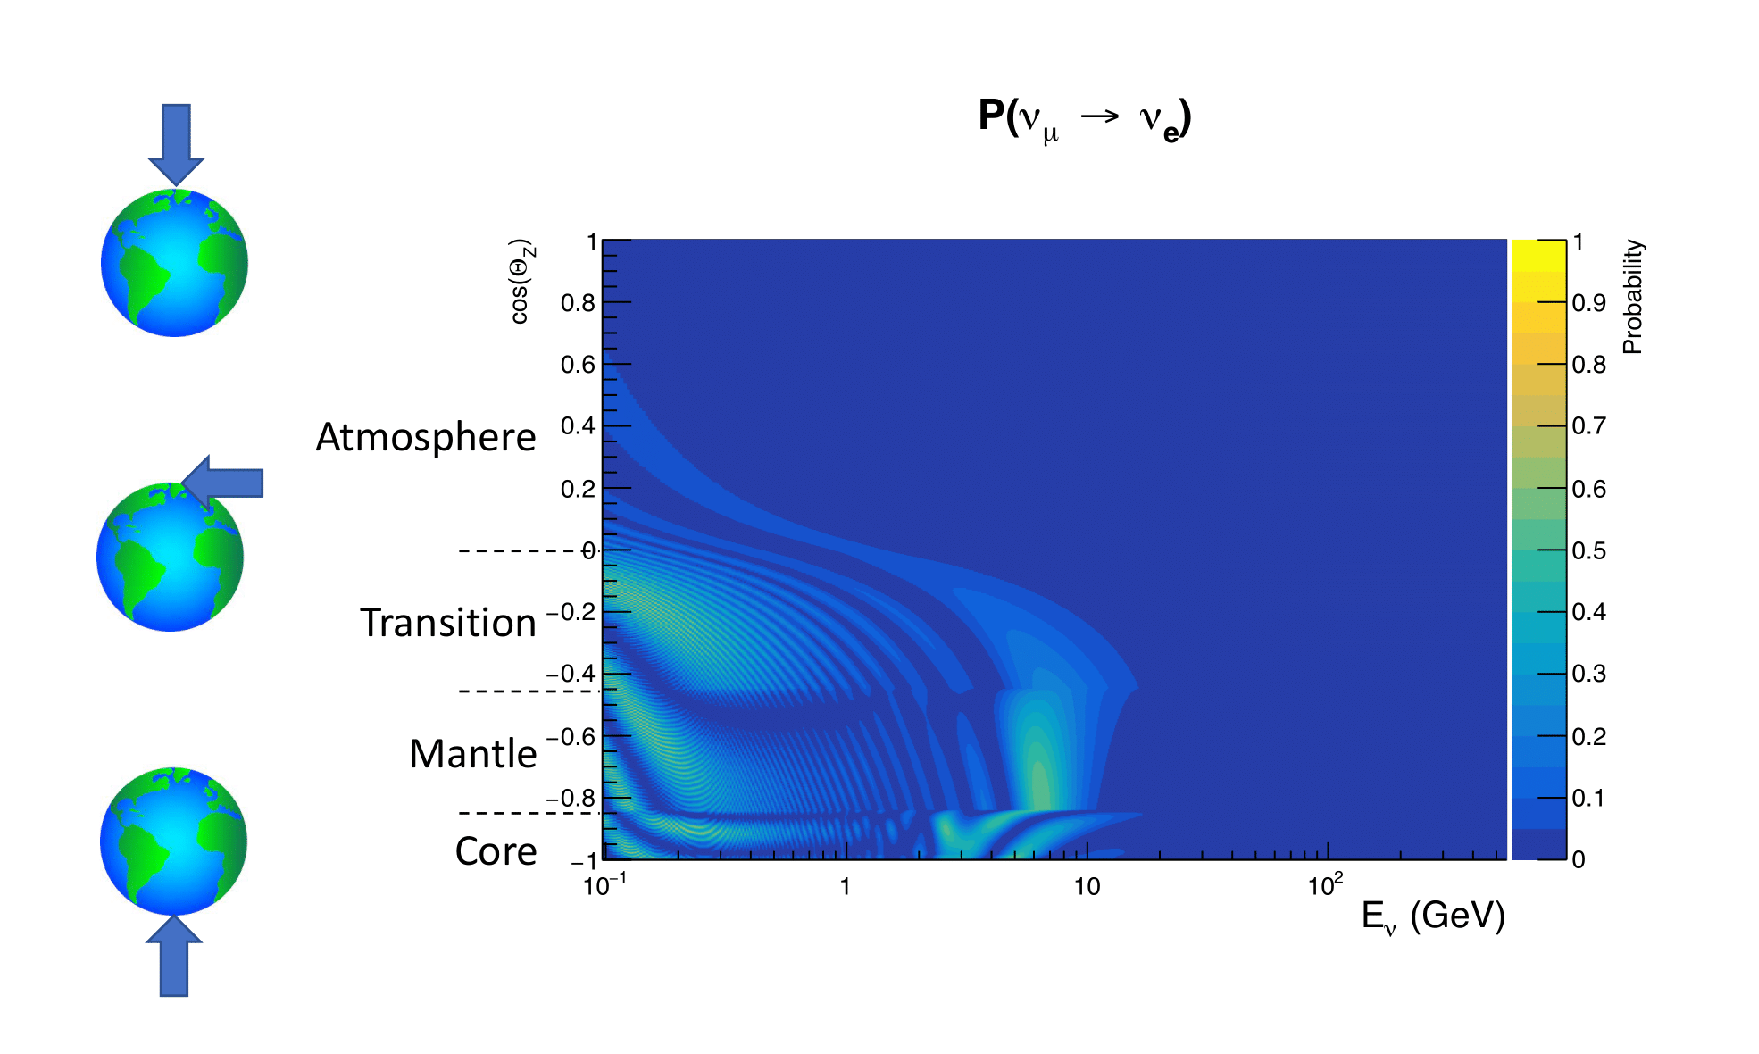
\includegraphics[width=\textwidth, trim={0mm 0mm 0mm 0mm}, clip,page=1]{Figures/Oscillation/BasicOscillogramWithNotes.pdf}
  \end{subfigure}
  \caption{An ``oscillogram'' that depicts the \quickmath{P(\nu_\mu \rightarrow \nu_e)} oscillation probability as a function of neutrino energy and cosine of the zenith angle. The zenith angle is defined such that \quickmath{\cos(\theta_{Z}) = 1.0} represents neutrinos that travel from directly above the detector. The four-layer constant density PREM model approximation is used and Asimov A oscillation parameters are assumed (\autoref{tab:Theory_ParameterSets}).}
  \label{fig:Oscillation_SK_BasicOscillogram}
\end{figure}

Atmospheric neutrinos have sensitivity to \quickmath{\delta_{CP}} through the overall event rate. \autoref{fig:Oscillation_SK_DCPSensitivity} illustrates the difference in oscillation probability between CP-conserving (\quickmath{\delta_{CP} = 0.}) and a CP-violating (\quickmath{\delta_{CP} = -1.601}) value taken from Asimov A oscillation parameter set (\autoref{tab:Theory_ParameterSets}). The result is a complicated oscillation pattern in the appearance probability for sub-GeV upgoing neutrinos. The detector does not have sufficient resolution to resolve these individual patterns so the sensitivity to \quickmath{\delta_{CP}} for atmospheric neutrinos comes via the overall normalisation of these events.

The presence of matter means that the effect \quickmath{\delta_{CP}} has on the oscillation probability is not equal between neutrinos and antineutrinos. Furthermore, the interaction cross-section for neutrinos is larger than for antineutrinos so the two effects have to be disentangled. These effects are further convoluted by detector efficiencies as SK cannot distinguish neutrinos and antineutrinos well. All of these effects lead to a difference in the number of neutrinos detected compared to antineutrinos. This changes how the \quickmath{\delta_{CP}} normalisation term is observed, resulting in a very complex sensitivity to \quickmath{\delta_{CP}}.

\begin{figure}[h]
  \begin{subfigure}[t]{\textwidth}
    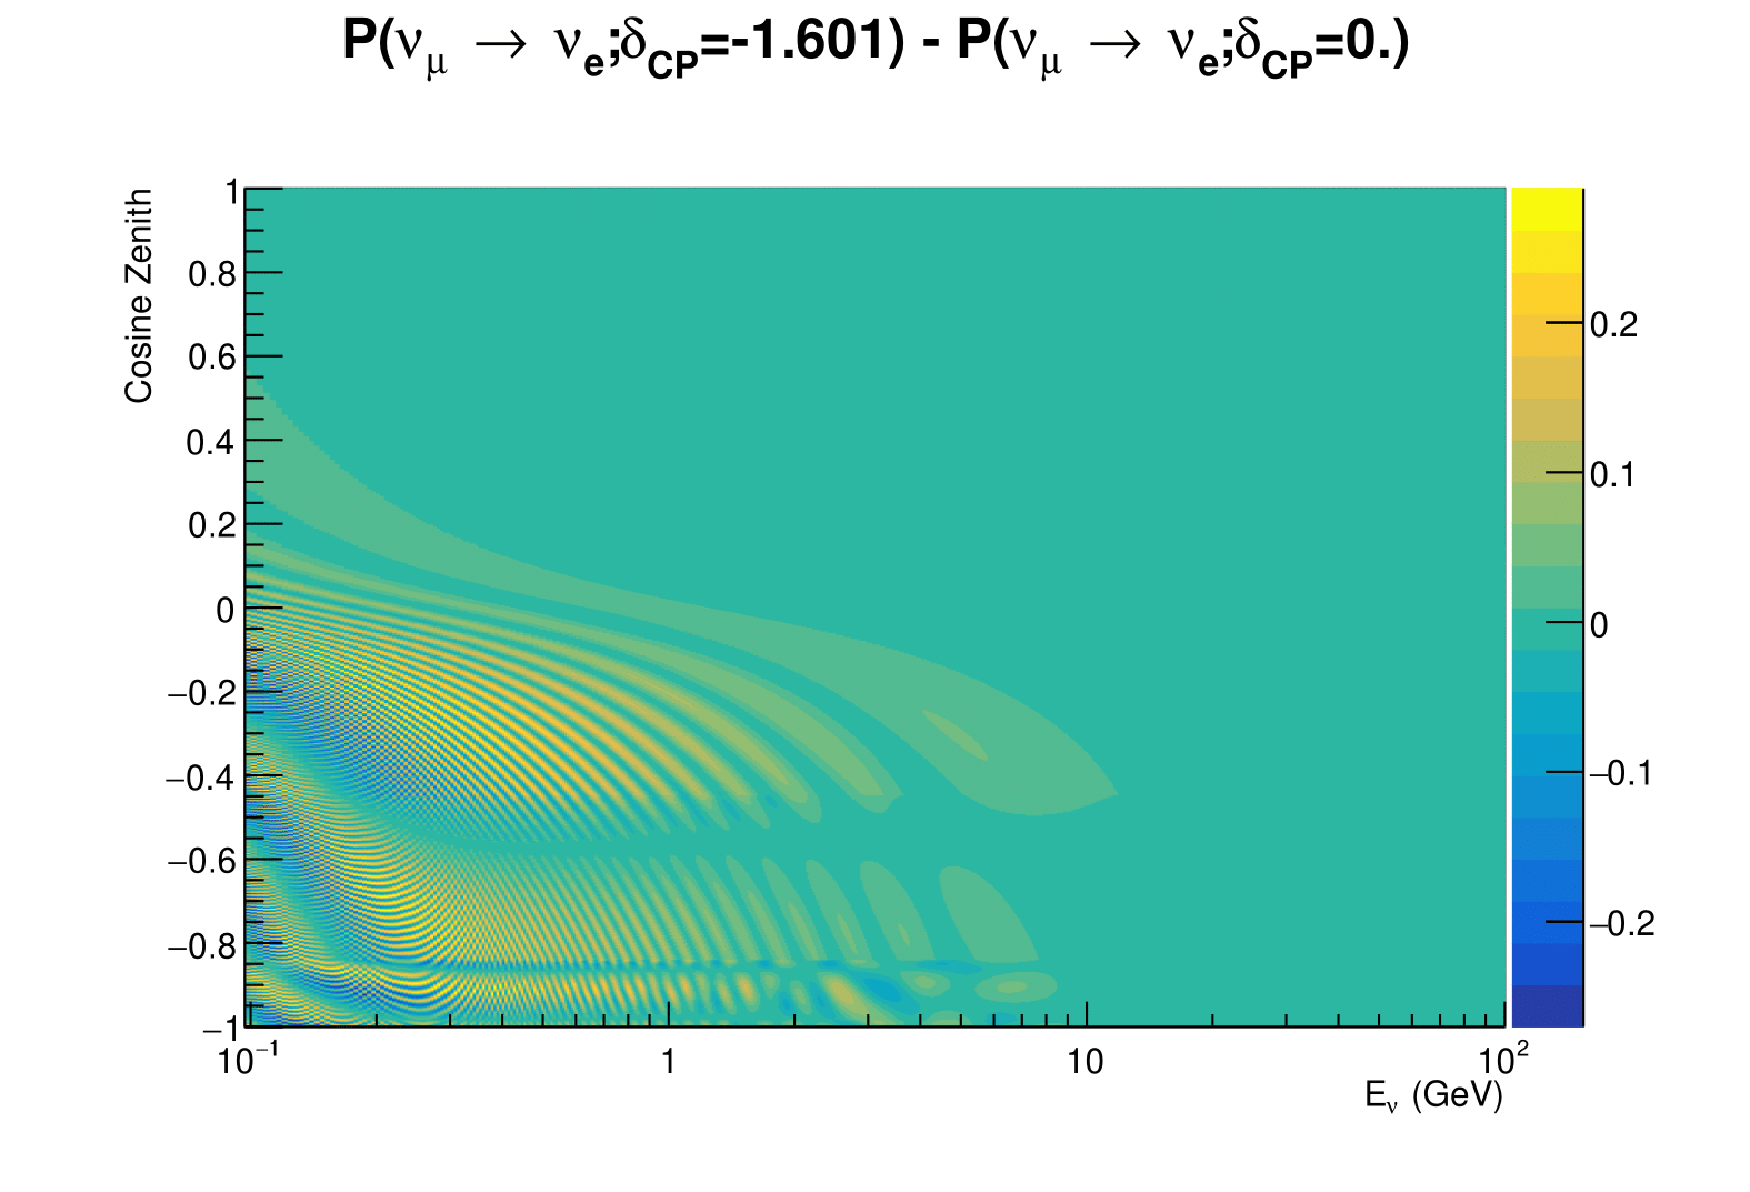
\includegraphics[width=\textwidth, trim={0mm 0mm 0mm 0mm}, clip,page=1]{Figures/Oscillation/AtmDCPSens.pdf}
  \end{subfigure}
  \caption{The effect of \quickmath{\delta_{CP}} for atmospheric neutrinos given in terms of the neutrino energy and zenith angle. This oscillogram compares the \quickmath{P(\nu_{\mu} \rightarrow \nu_{e})} oscillation probability for a CP conserving (\quickmath{\delta_{CP}=0.0}) and a CP violating (\quickmath{\delta_{CP}=-1.601}) value taken from the Asimov A parameter set. The other oscillation parameters assume the Asimov A oscillation parameter set given in \autoref{tab:Theory_ParameterSets}.}
  \label{fig:Oscillation_SK_DCPSensitivity}
\end{figure}

The vacuum and matter oscillation probabilities for \quickmath{P(\nu_{e} \rightarrow \nu_{e})} and \quickmath{P(\bar{\nu}_{e} \rightarrow \bar{\nu}_{e})} are presented in \autoref{fig:Oscillation_SK_VacuumMatter}, where the PREM model has been assumed. The oscillation probability for both neutrinos and antineutrinos is affected in the presence of matter. However, the resonance effects around \quickmath{O(5)\text{GeV}} only occur for neutrinos in the normal mass hierarchy and antineutrinos in the inverse mass hierarchy. The exact position and amplitude of the resonance depend on \quickmath{\sin^{2}(\theta_{23})}, further increasing the atmospheric neutrinos' sensitivity to the parameter.

\begin{figure}[h]
  \begin{subfigure}[t]{\textwidth}
    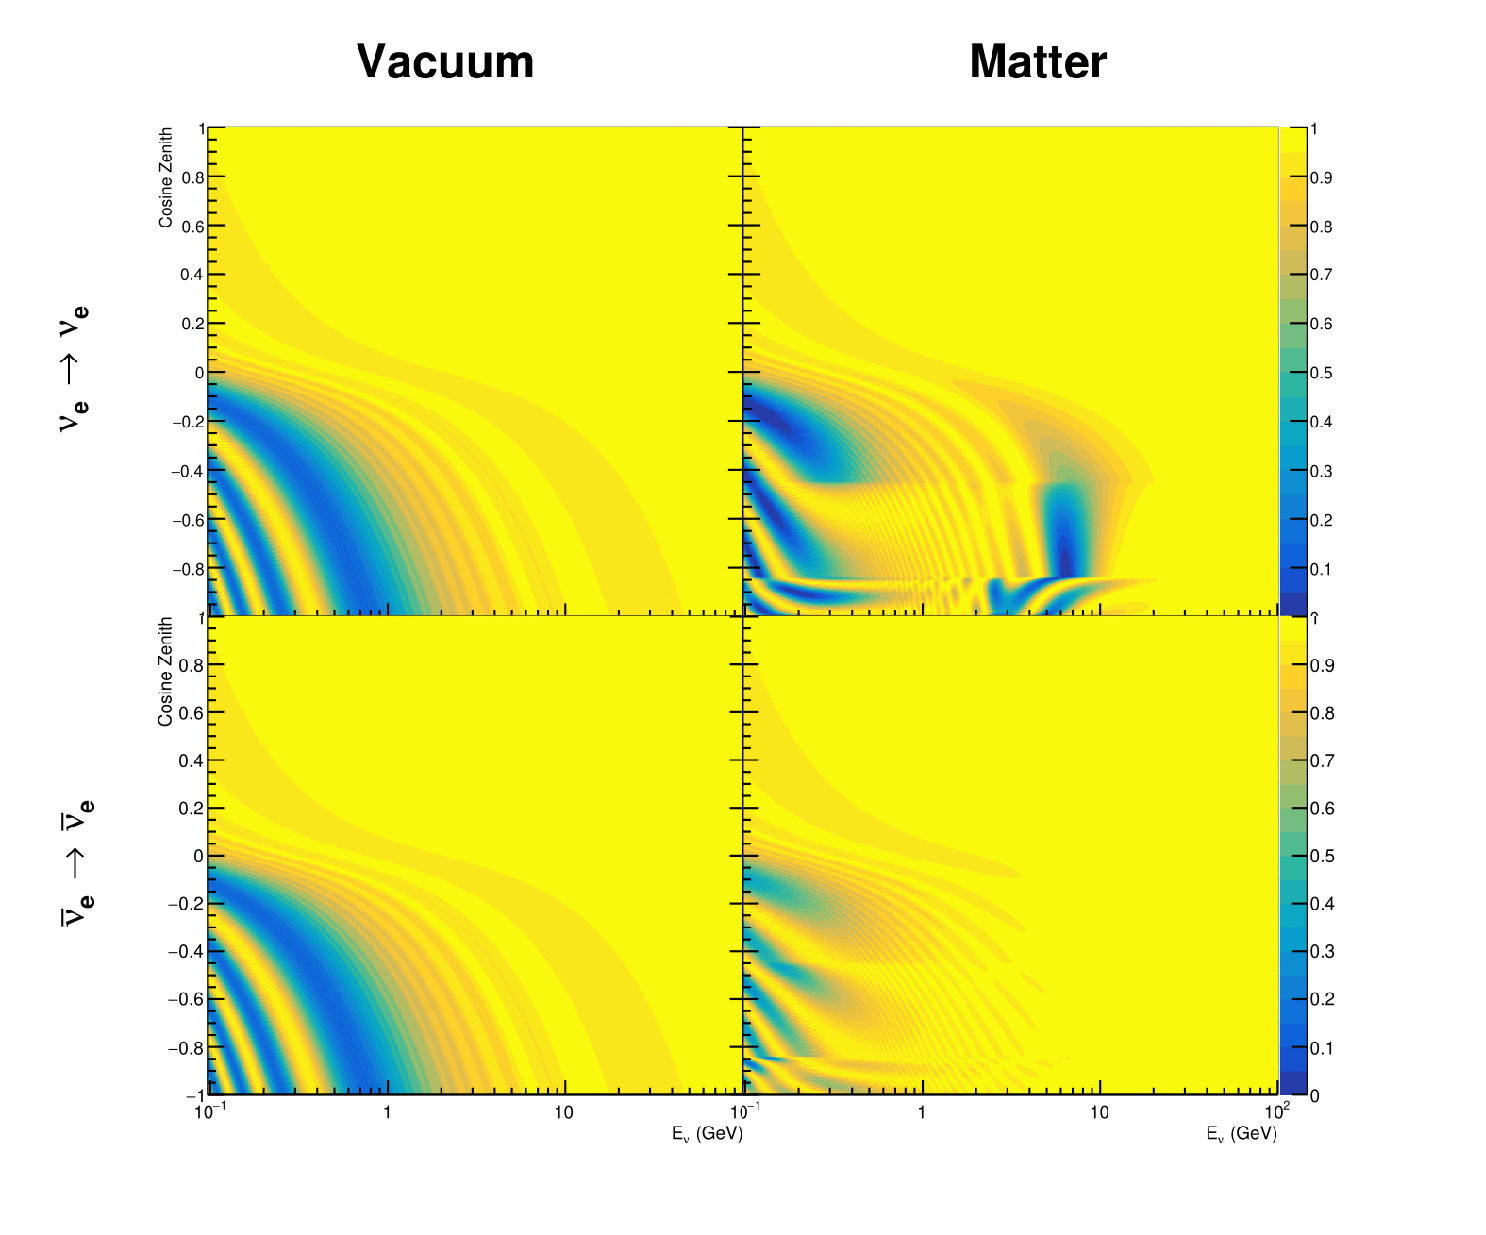
\includegraphics[width=\textwidth, trim={0mm 0mm 0mm 0mm}, clip,page=1]{Figures/Oscillation/MatterEffect.pdf}
  \end{subfigure}
  \caption{An illustration of the matter-induced effects on the oscillation probability, given as a function of neutrino energy and zenith angle. The top row of panels gives the \quickmath{P(\nu_{e} \rightarrow \nu_{e})} oscillation probability and the bottom row illustrates the \quickmath{P(\bar{\nu}_{e} \rightarrow \bar{\nu}_{e})} oscillation probability. The left column highlights the oscillation probability in a vacuum, whereas the middle and right column represents the oscillation probabilities when the four-layer fixed density PREM model is assumed. All oscillation probabilities assume the ``Asimov A'' set given in \autoref{tab:Theory_ParameterSets}, but importantly, the right column sets an inverted mass hierarchy. The ``matter resonance'' effects at \quickmath{E_{\nu} \sim 5\text{GeV}} can be seen in the \quickmath{P(\nu_{e} \rightarrow \nu_{e})} for normal mass hierarchy and \quickmath{P(\bar{\nu}_{e} \rightarrow \bar{\nu}_{e})} for inverted hierarchy.}
  \label{fig:Oscillation_SK_VacuumMatter}
\end{figure}

As the T2K beam flux is centered at the first oscillation maximum (\quickmath{E_{\nu} = 0.6\text{GeV}}) \cite{t2k_det}, the sensitivity to \quickmath{\delta_{CP}} is predominantly observed as a change in the event-rate of e-like samples in \quickmath{\nu/\bar{\nu}} modes. \autoref{fig:Oscillation_T2K_OscillationProbSensitivity} illustrates the \quickmath{P(\nu_\mu \rightarrow \nu_e)} oscillation probability for a range of \quickmath{\delta_{CP}} values. %The magnitude of the oscillation peak has an approximate factor of two difference between the CP-violating values \quickmath{\delta_{CP} = \pm\pi/2} and the difference in oscillation probability between the CP-conserving
A circular modulation of the first oscillation peak (in both magnitude and position) is observed when varying throughout the allowable values of \quickmath{\delta_{CP}}. The CP-conserving values of \quickmath{\delta_{CP}=0,\pi} have a lower(higher) oscillation maximum than the CP-violating values of \quickmath{\delta_{CP}=-\pi/2}(\quickmath{\delta_{CP}=\pi/2}). A sub-dominant shift in the energy of the oscillation peak is also present, which aids in separating the two CP-conserving values of \quickmath{\delta_{CP}}.

\begin{figure}[h]
  \begin{subfigure}[t]{0.5\textwidth}
    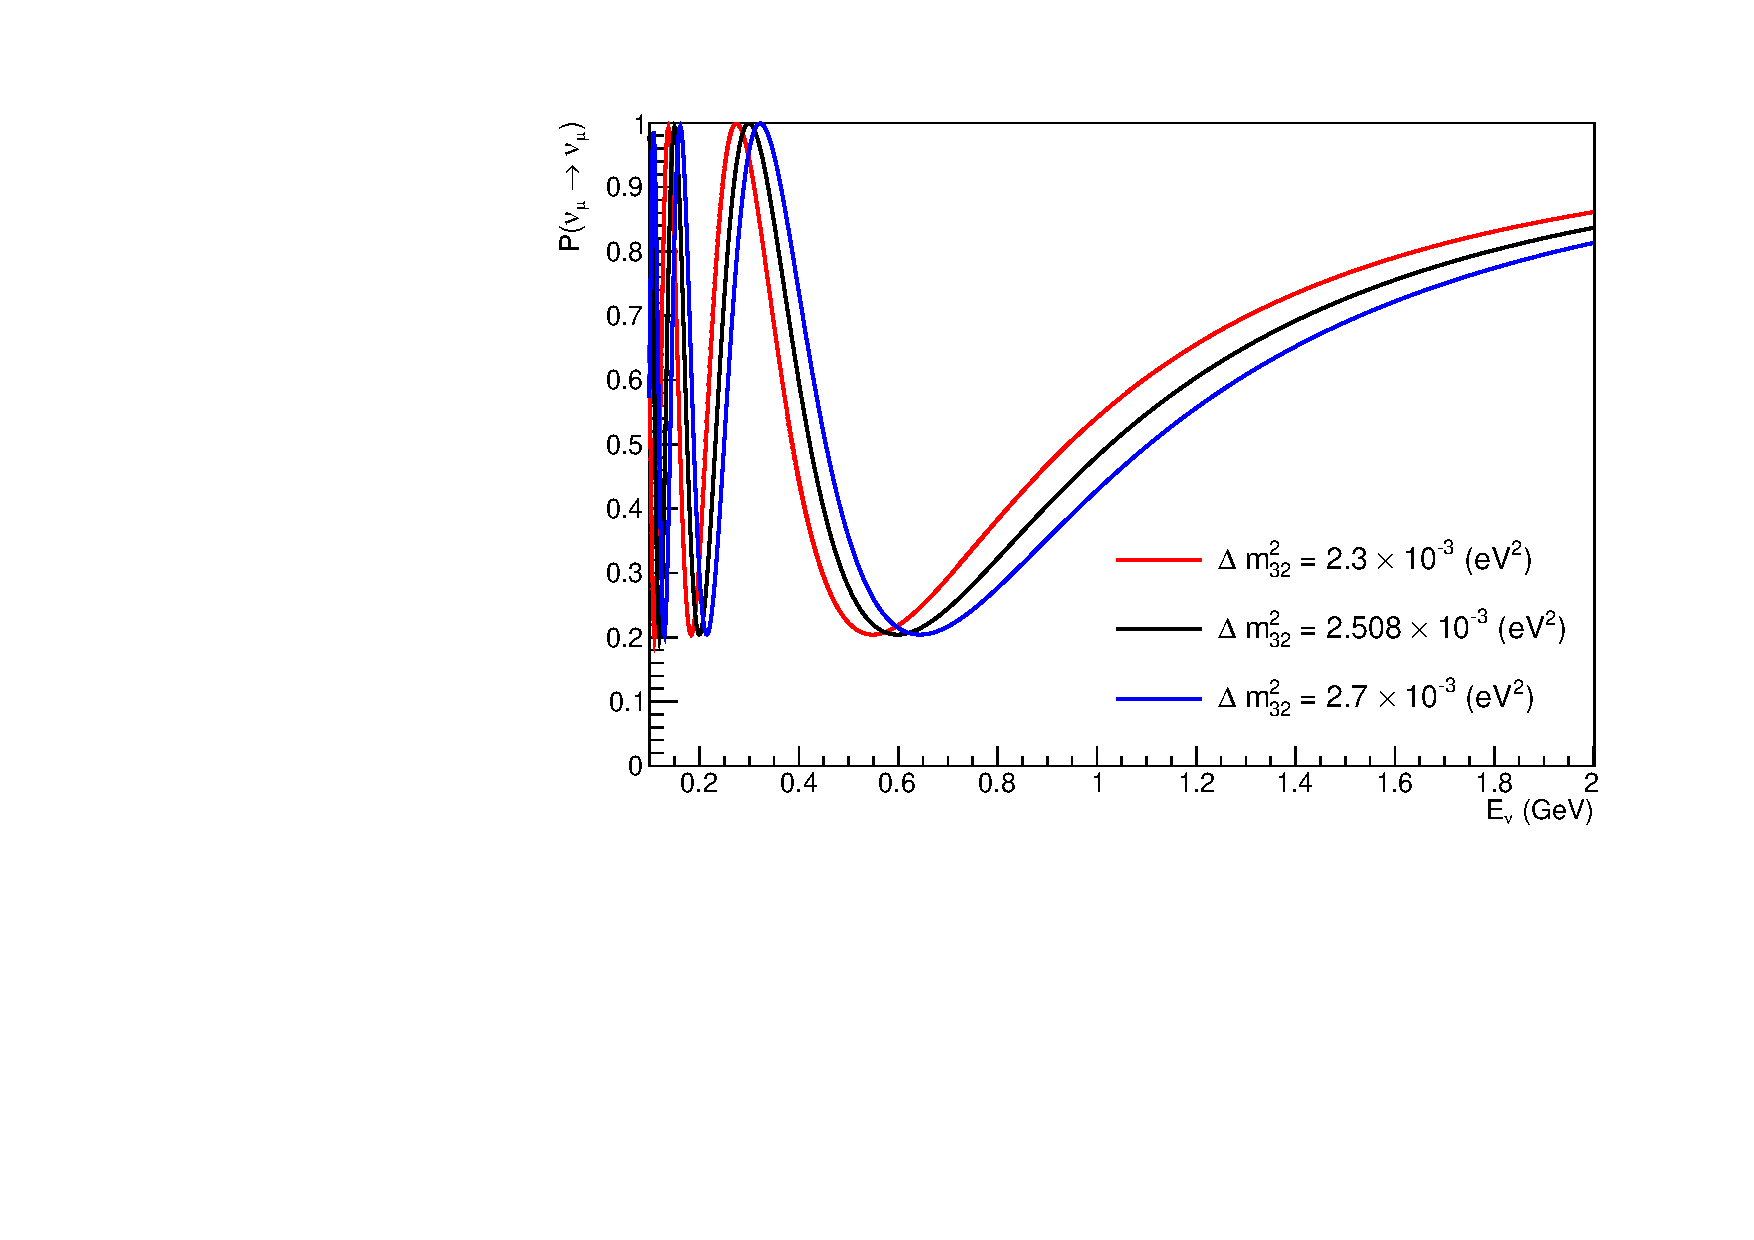
\includegraphics[width=\textwidth, trim={0mm 0mm 0mm 0mm}, clip,page=1]{Figures/Oscillation/T2K_NuMu_x_NuMu_DelMsq32Sens.pdf}
    \subcaption{\quickmath{\Delta m^{2}_{32}}}
  \end{subfigure}%
  \begin{subfigure}[t]{0.5\textwidth}
    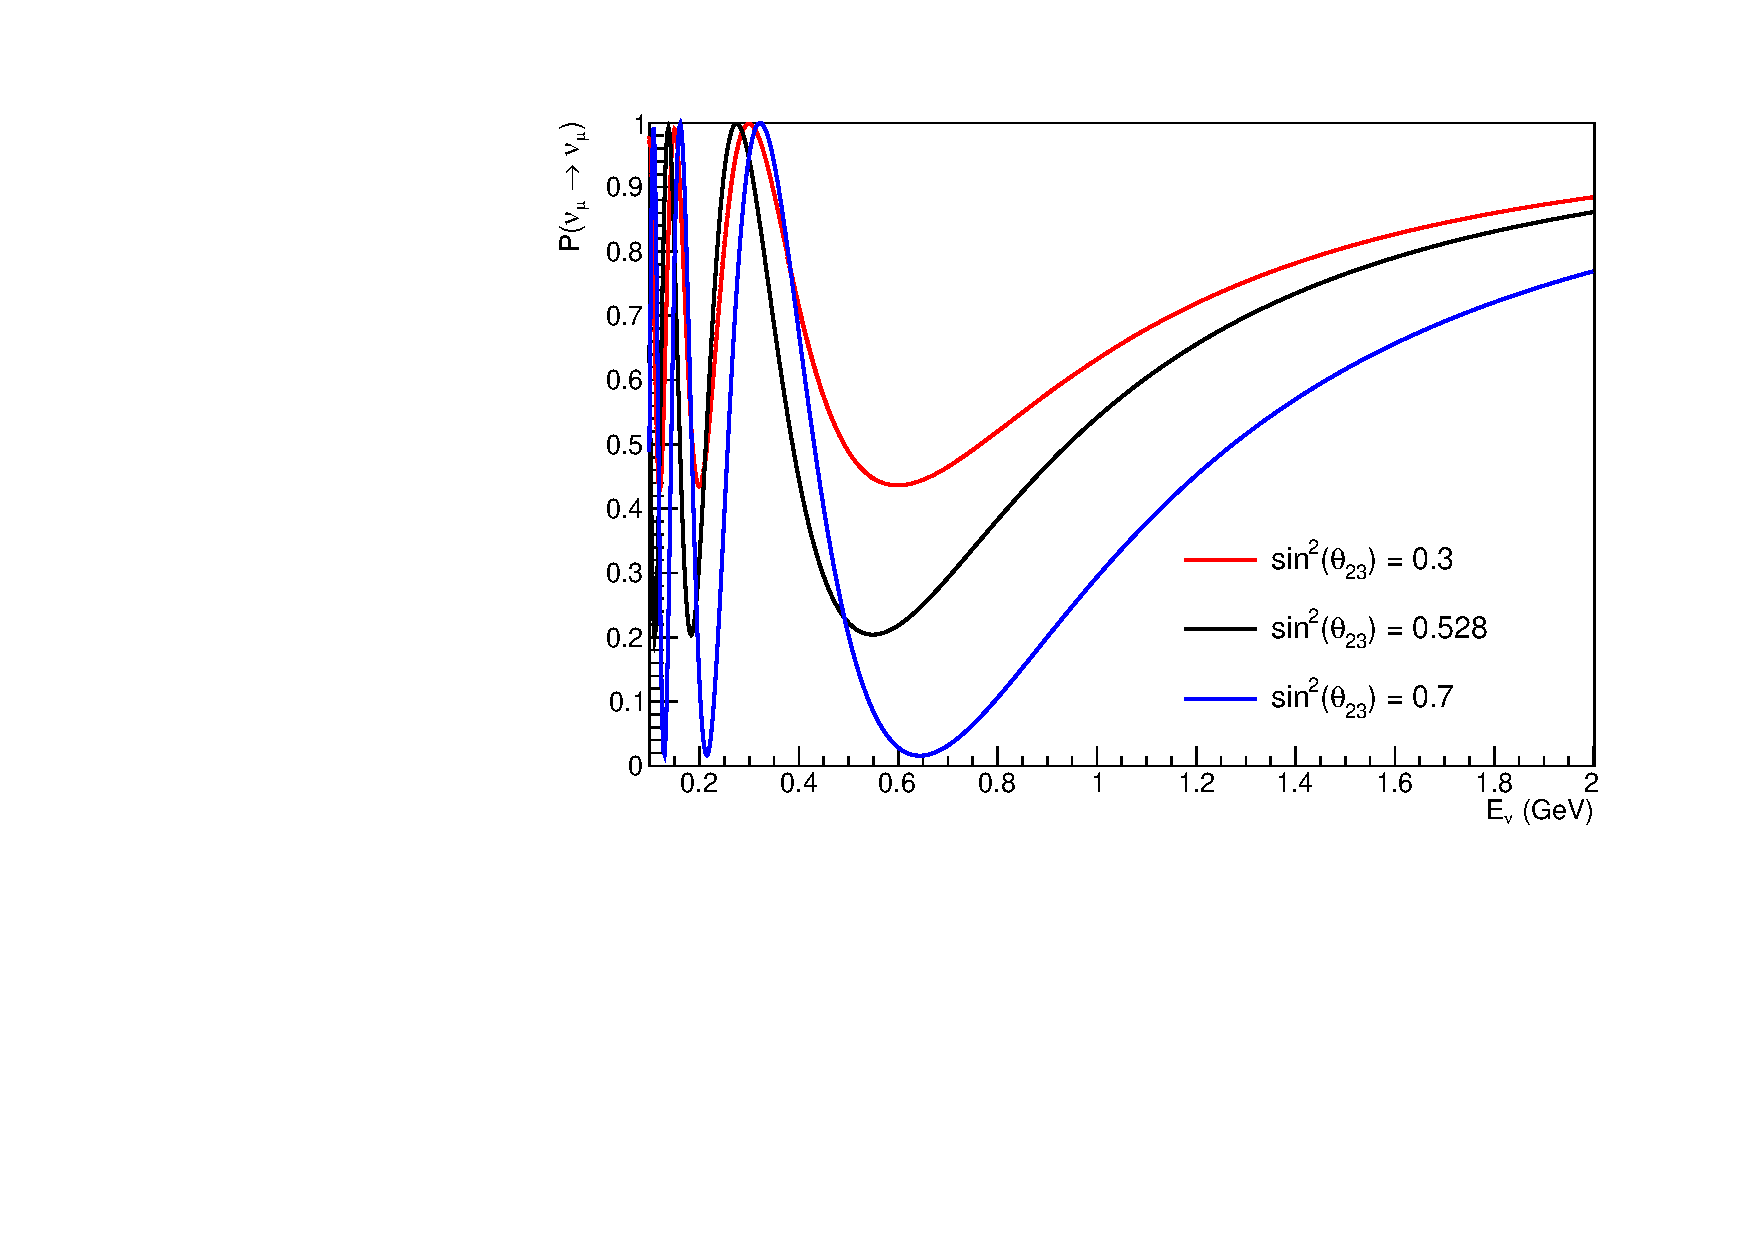
\includegraphics[width=\textwidth, trim={0mm 0mm 0mm 0mm}, clip,page=1]{Figures/Oscillation/T2K_NuMu_x_NuMu_Sinsqth23Sens.pdf}
    \subcaption{\quickmath{\sin^{2}(\theta_{23})}}
  \end{subfigure}
  \begin{subfigure}[t]{0.5\textwidth}
    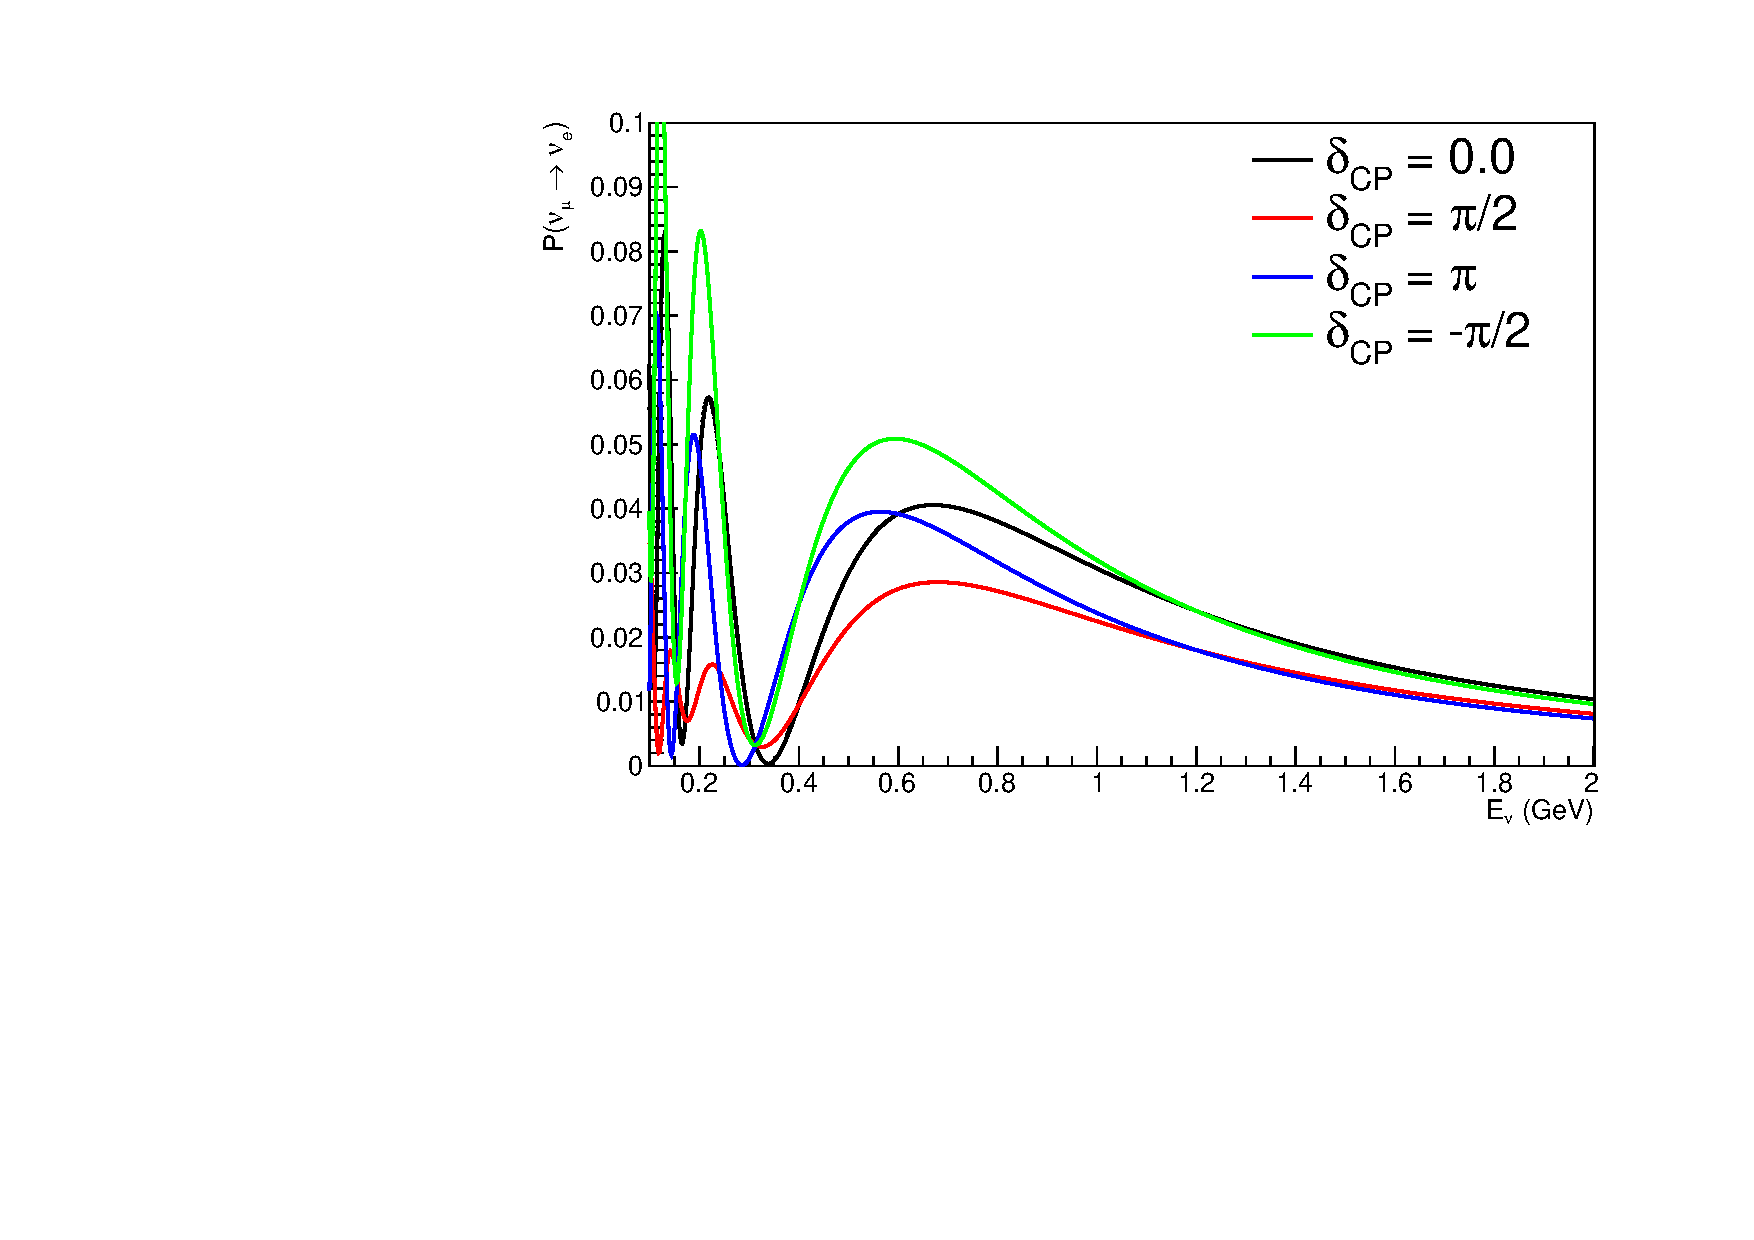
\includegraphics[width=\textwidth, trim={0mm 0mm 0mm 0mm}, clip,page=1]{Figures/Oscillation/T2K_NuMu_x_NuE_DCPSens.pdf}
    \subcaption{\quickmath{\delta_{CP}}}
  \end{subfigure}
  \caption{The oscillation probability for beam neutrino events given as a function of neutrino energy. All oscillation parameters assume the ``Asimov A'' set given in \autoref{tab:Theory_ParameterSets} unless otherwise stated. Each panel represents a change in one of the oscillation parameters whilst keeping the remaining parameters fixed.}
  \label{fig:Oscillation_T2K_OscillationProbSensitivity}
\end{figure}

T2K's sensitivity to \quickmath{\sin^{2}(\theta_{23})} and \quickmath{\Delta m^{2}_{32}} is observed as a shape-based variation of the muon-like samples, as illustrated in \autoref{fig:Oscillation_T2K_OscillationProbSensitivity}. The value of \quickmath{\Delta m^{2}_{32}} laterally shifts the position of the oscillation dip (around \quickmath{E_\nu \sim 0.6\text{GeV}}) in the \quickmath{P(\nu_\mu \rightarrow \nu_\mu)} oscillation probability. A variation of \quickmath{\sin^{2}(\theta_{23})} is predominantly observed as a vertical shift of the oscillation dip with second-order horizontal shifts being due to matter effects. The beam neutrinos have limited sensitivity to matter effects due to the relatively shorter baseline as well as the Earth's mantle being a relatively low-density material (as compared to the Earth's core). For some values of \quickmath{\delta_{CP}}, the degeneracy in the number of e-like events allows the mass hierarchy to be broken. This leads to a \quickmath{\delta_{CP}}-dependent mass hierarchy sensitivity which can be seen in \autoref{fig:Oscillation_SK_BiProbabilityPlot}.

\begin{figure}[h]
  \begin{subfigure}[t]{0.65\textwidth}
    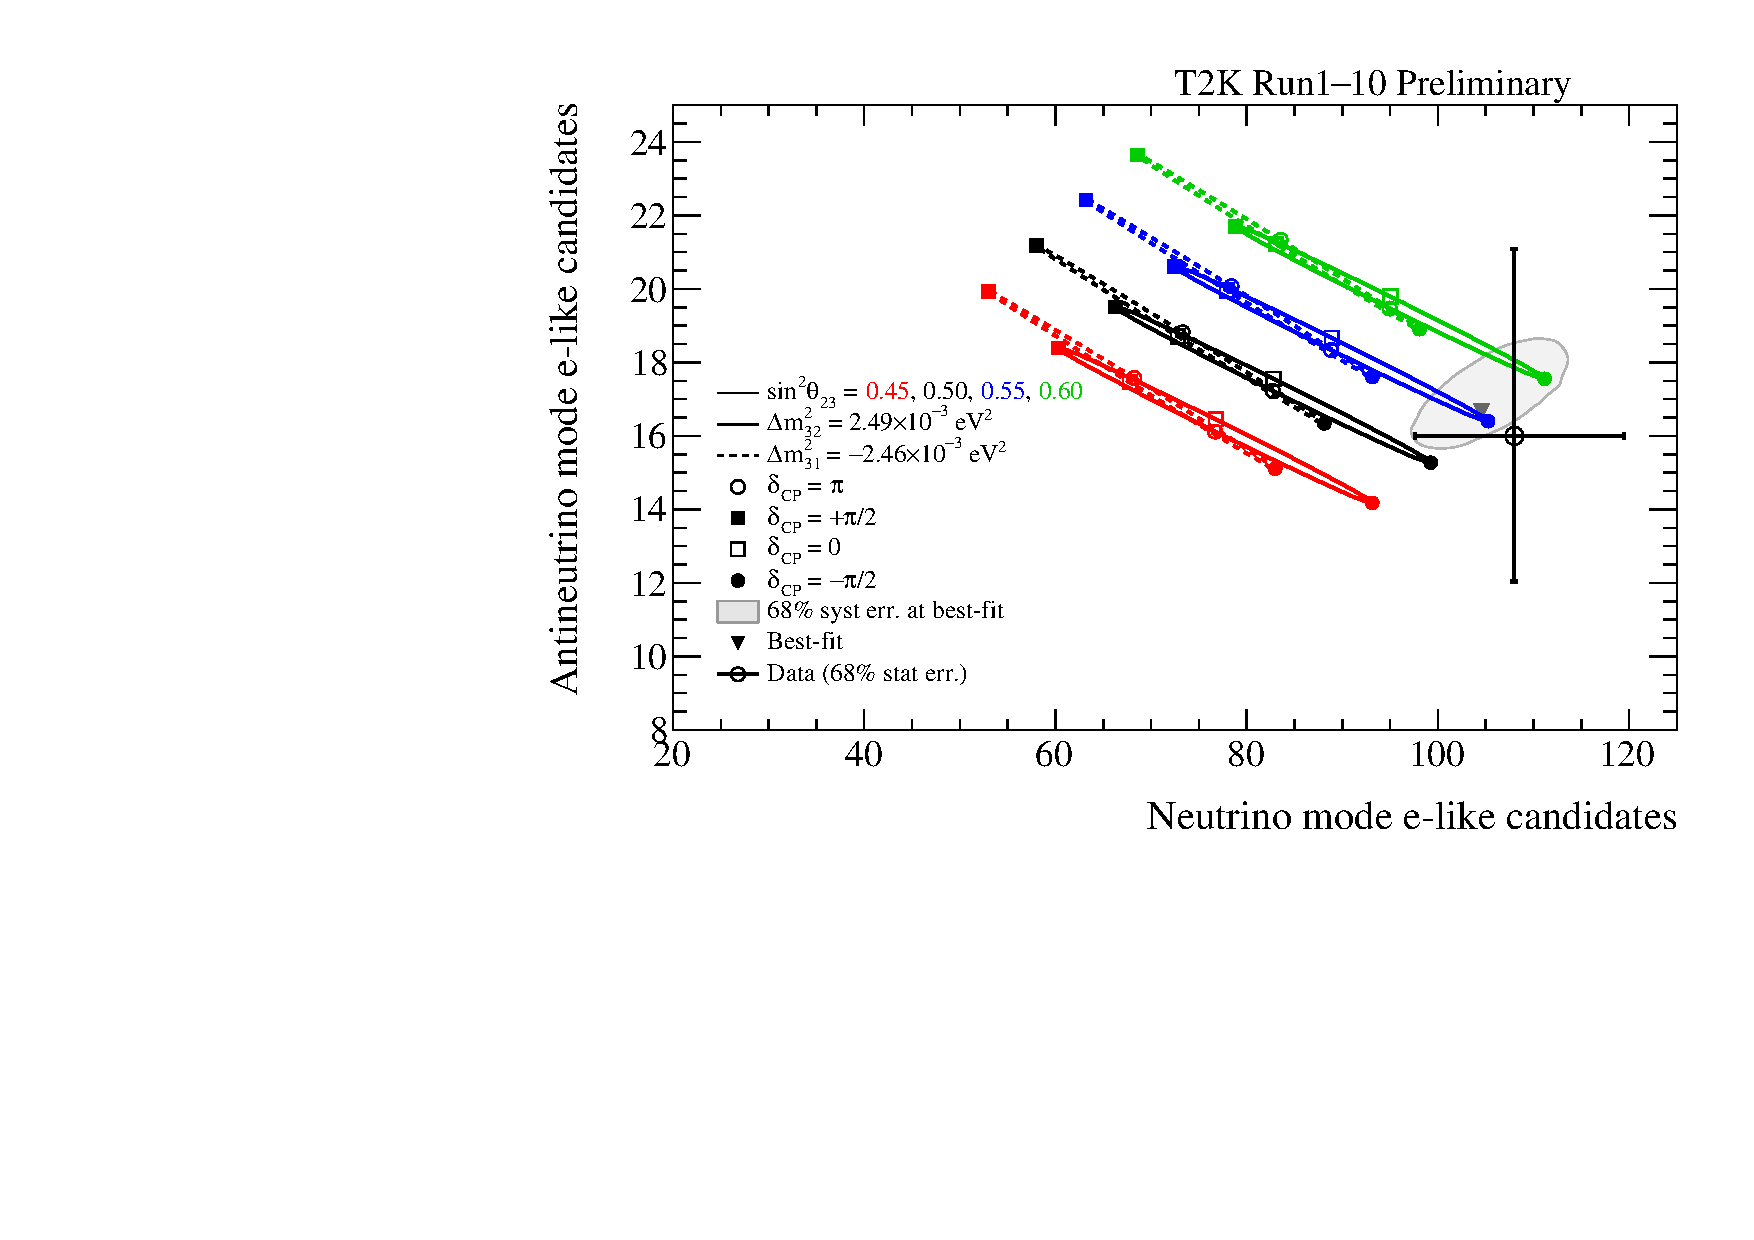
\includegraphics[width=\textwidth, trim={0mm 0mm 0mm 0mm}, clip,page=1]{Figures/Oscillation/BiProbabilityPlot.pdf}
  \end{subfigure}
  \caption{The number of electron-like events in the FHC and RHC operating mode of the beam, as a function of the oscillation probabilities. Both normal hierarchy (Solid)) and inverse hierarchy (Dashed) values of \quickmath{\Delta m^{2}_{32}} are given.}
  \label{fig:Oscillation_SK_BiProbabilityPlot}
\end{figure}

Whilst all oscillation channels should be included for completeness, the computational resources required to run a fit are limited and any reasonable approximations which reduce the number of oscillation probability calculations that need to be made should be applied. The \quickmath{\nu_{e} \rightarrow \nu_{e,\mu,\tau}} (and antineutrino equivalent) oscillations can be ignored for beam neutrinos as the \quickmath{\nu_{e}/\bar{\nu}_{e}} fluxes are approximately two orders of magnitude smaller than the corresponding \quickmath{\nu_{\mu}/\bar{\nu}_{\mu}} flux. Furthermore, as the peak neutrino energy of the beam is well below the threshold for charged current tau production (\quickmath{E_\nu = 3.5\text{GeV}} \cite{Li_2018}), only a small proportion of the neutrinos produced in the beam have the required energy. For the few neutrinos that have sufficient energy, the oscillation probability is very small due to their energy being well above the oscillation maximum (small value of \quickmath{L/E}). Whilst these approximations have be made for the beam neutrinos, the atmospheric flux of \quickmath{\nu_{e}} is of the same order of magnitude as the \quickmath{\nu_{\mu}} flux and the energy distribution of atmospheric neutrinos extends well above the tau production threshold. These events can have non-negligible oscillation probabilities due to the further distance they travel.
